\documentclass{iopart}
%\documentclass[12pt]{article}

\usepackage{url}
\usepackage{amsbsy}
\usepackage{graphicx}
\input{epsf} 

\begin{document}



\title
{First results of scientific performance for the design of ESA space based gravitational wave detector ({\it ELISA}) }

\author{The \emph{Parameter Estimation Task Force}:
Pau Amaro-Seoane$^1$,
Sofiane Aoudia$^1$,
G\'erard Auger$^2$,
Stanislav Babak$^1$,
Emanuele Berti$^3$
Neil J. Cornish$^4$,
Jonathan Gair$^5$,
Ryan Lang$^6$,
Tyson Littenberg$^6$,
Sean McWilliams$^6$,
Oliver Jennrich$^7$,
Philippe Jetzer$^8$,
Ioannis Kamaretsos$^9$,
Antoine Klein$^8$,
Gijs Nelemans$^{10}$,
Frank Ohme$^1$,
Eric Plagnol$^2$,
Antoine Petiteau$^1$,
Edward K. Porter$^2$,
Emma Robinson$^1$,
B. S. Sathyaprakash$^9$,
Bernard Schutz$^1$,
Alberto Sesana$^1$,
Carlos Sopuerta$^{11}$,
Alessandro Spallicci$^{12}$,
Ira Thorpe$^6$,
Michele Vallisneri$^{13,14}$,
Alberto Vecchio$^{15}$,
Marta Volonteri$^{16}$
}

\address{$^1$ Max-Planck-Institut f\"ur Gravitationsphysik (Albert-Einstein-Institut), Am M\"uhlenberg 1, D-14476 Golm bei Potsdam, Germany}
\address{$^2$ APC, UMR 7164, Univ.\ Paris 7 Denis Diderot, 10, rue Alice Domon et Leonie Duquet, 75025 Paris Cedex 13, France}
\address{$^3$ University of Mississippi, USA}
\address{$^4$ Dept.\ of Physics, Montana State Univ., Bozeman, MT 59717, USA}
\address{$^5$ Inst.\ of Astronomy, Univ.\ of Cambridge, Madingley Rd., Cambridge, CB30HA, UK}
\address{$^6$ Gravitational Astrophysics Lab., NASA Goddard Space Flight Center, 8800 Greenbelt Rd., Greenbelt, MD 20771, USA}
\address{$^7$ European Space Agency}
\address{$^8$ Institute of Theoretical Physics, University of Zurich}
\address{$^9$ School of Physics and Astronomy, Cardiff Univ., 5, The Parade, Cardiff, CF243YB, UK}
\address{$^{10}$ Department of Astrophysics, Radboud University Nijmegen, The Netherlands}
\address{$^{11}$ Institute of Space Sciences (ICE-CSIC), Barcelona, Spain}
\address{$^{12}$ University of Orleans, France}
\address{$^{13}$ Jet Propulsion Laboratory, California Inst.\ of Technology, Pasadena, CA 91109, USA}
\address{$^{14}$ Theoretical Astrophysics, California Inst.\ of Technology, Pasadena, CA 91125}
\address{$^{15}$ School of Physics and Astronomy, Univ.\ of Birmingham, Edgbaston, Birmingham B152TT, UK}
\address{$^{16}$ University of Michigan}

\ead{Antoine.Petiteau@aei.mpg.de, porter@apc.univ-paris7.fr}


\begin{abstract}

This document collects the current results of 

\end{abstract}



%Uncomment for PACS numbers title message

%\pacs{00.00, 20.00, 42.10}



% Uncomment for Submitted to journal title message

%\submitto{\JPA}\



% Comment out if separate title page not required

\maketitle

\tableofcontents

%%%%%%%%%%%%%%%%%%%%%%%%%%%%%%%%%%%%%
%                                                       Instrument                                                      %
%%%%%%%%%%%%%%%%%%%%%%%%%%%%%%%%%%%%%
\section{ Instrument configurations : noises, orbits and sensitivity }
\label{S:Instrument}
{\it ('section captain' : Antoine Petiteau)}


\subsection{Overview}
\label{SS:Inst:Overview}

During the "first phase" (before CDF), 6 configurations had been defined. The table \ref{T:Configs} gives a summary of their main characteristics and the induced noise levels.

\begin{table}[htdp]
\begin{center}
\begin{tabular}{|c|c|c|c|c|c|c|}
\hline
Configuration 				& C5 	& C4	 	& C3 	& C2 	& C1  	& HL1 	\\
\hline
Armlength ($\times 10^9 $ m) 	& 2 		& 3 		& 1		& 1		& 1 	  	&  1 - 1.6 		\\
Orbits					& analytic & analytic & analytic & $10^o$ & closest 	& $20^o$ \\
\hline
Diameter telescope (m) 		& 0.28 	& 0.25 	& 0.25	& 0.4		& 0.4 	&  0.25 	\\
Laser power (W) 			& 2	 	& 0.7 	& 0.7		& 2		& 0.05 	&  0.7 		\\
Acceleration system 			& DRS	& DRS 	& DRS	& DRS	& LPF$^{(1)}$	&  DRS 	\\
\hline
Acceleration ($ 10^{-48} f^{-2} \textrm{Hz}^{-1}$)  & 6	&  6	& 6	& 6	&  $8.2\left( 1 + {  1.8 \times 10^4 \over f^2 }  \right) ^ 2 $	&   6 \\  %2.54	\\
Shot noise ($ 10^{-38} f^{2}  \textrm{Hz}^{-1}$)  &  2.05 &  20.07 &  2.31 & 0.06$^{(2)}$  & 4.92 & 2.31 \\ %11.2 \\
Fixed noise ($10^{-38} f^{2} \textrm{Hz}^{-1}$)  &  2.81 &  2.81 &  2.81 & 2.81  & 2.81 &  2.81 \\ %6.32 \\
\hline
\end{tabular}
\end{center}
\caption{Summary of configuration. Noises are given in $\delta \nu / \nu$ unit. \\ 
{ \scriptsize Notes about particular cases including mistakes : ${(1)}$ the margin has been taken into account 2 times  ; 
${(2)}$ the laser power has been considered in the rms shot noise  with power -1 instead of -0.5 . } }
\label{T:Configs}
\end{table}%


\subsection{Noises}
\label{SS:Inst:Noises}
The noise models used for the new space-based gravitational wave detector supported by ESA have been provided by ESA.
Each noise includes the standard ESA margin $M_{ESA} = 1 / 0.65 $ .

In the following description, we give the general formulation of the root mean square value (RMS), i.e. square root of the power spectral density (PSD) in the standard unit of the noise. 
We also give the value used for each configurations in relative frequency unit $\delta \nu \over \nu$.

The conversion between rms noise, $\delta x$,  and power spectral density $S$ is : $S = \delta x ^ 2$.

The conversion between acceleration noise unit (in $\textrm{m}^2.\textrm{s}^{-4}.\textrm{Hz}^{-1}$) and noise in length unit (in $\textrm{m}^2.\textrm{Hz}^{-1}$) is :
\begin{equation}
S(f) =  S_{\textrm{m}^2.\textrm{s}^{-4}.\textrm{Hz}^{-1}}(f) / (2 \pi f)^4 \;  \textrm{m}^2.\textrm{Hz}^{-1}
\end{equation}
 
The conversion between  noise in length unit ($\textrm{m}^2.\textrm{Hz}^{-1}$) and noise in relative frequency unit (in $\textrm{Hz}^{-1}$) is :
\begin{equation}
S_{\delta \nu \over \nu}(f) =  S (f) \times \left( {2 \pi f \over c } \right)^2 \;  \textrm{Hz}^{-1}
\end{equation}

 

\subsubsection{Acceleration noises}
\label{SSS:Inst:Noises:Acc}
This noise is due to the limitation of the drag-free system. 
We consider two types of acceleration noise : 
\begin{itemize}
\item DRS : acceleration noise corresponding to LISA requirements :
\begin{equation}
\delta x_{\textrm{acc}}^{\textrm{DRS}} =  M_{ESA} \times 3 \times 10^{-15}  \textrm{m}/\textrm{s}^2/\sqrt{\textrm{Hz}} 
\end{equation}

\item LPF  : acceleration noise corresponding to LISAPathfinder :
\begin{equation}
\delta x_{\textrm{acc}}^{\textrm{LPF}} = M_{ESA} \times 3.5 \times 10^{-15} \left( 1 + { 0.18 \ \textrm{mHz} \over f }  \right) \textrm{m}/\textrm{s}^2/\sqrt{\textrm{Hz}}
\end{equation}

\end{itemize}

So, we have one best case, the DRS, and one worth case, the LPF. 

Note that for the LPF noise, we include the ESA margin but, according to Stefano Vitale, the margin was already taken into account in the   $3.5 \times 10^{-15}$ value. So the LPF acceleration was over-estimated (only used for configuration C1).

The acceleration noise for the different configurations is :
\begin{itemize}
\item for C1 : 
\begin{equation}
S_{acc, {\delta \nu \over \nu}} (f)  =  8.17 \times 10^{-48} \left( { 1 \over f} + \left({1.8 \times 10^{-4} \over f ^2} \right) \right)^2 Hz^{-1}
\end{equation}
\item for C2, C3, C4, C5, HL1 :
\begin{equation}
S_{acc, {\delta \nu \over \nu}} (f)  =  6.00 \times 10^{-48} f^{-2} Hz^{-1}
\end{equation}
\end{itemize}
 






\subsubsection{Shot noise}
\label{SSS:Inst:Noises:Shot}

This noise depends directly on the received laser power after the travel between two spacecrafts. Therefore it depends on :
\begin{itemize}
\item $L$ : the armlength (in m ),
\item $D$ : the diameter of the telescope (in m),
\item $P$ : the emitted laser power (in Watt) 
\end{itemize}
 

\begin{equation}
\delta x,_{\textrm{SN}} = M_{ESA} \times  7.7 \times 10^{-12}  \left( {1 \ \textrm{W} \over P } \right)^{1/2} \left( { L \over 5 \times 10^9 \ \textrm{m}} \right) \left( {0.4 \ \textrm{m} \over D }\right)^2  \textrm{m}/\sqrt{\textrm{Hz}} 
\end{equation}


The acceleration noise for the different configurations is :
\begin{itemize}
\item for C1 : 
\begin{equation}
S_{SN, {\delta \nu \over \nu}} (f)  =  4.92 \times10^{-38} f^2 Hz^{-1}
\end{equation}
\item for C2 : 
\begin{equation}
S_{SN, {\delta \nu \over \nu}} (f)  =  6.14 \times10^{-40} f^2 Hz^{-1}
\end{equation}
\item for C3 : 
\begin{equation}
S_{SN, {\delta \nu \over \nu}} (f)  =  2.31 \times10^{-38} f^2 Hz^{-1}
\end{equation}
\item for C4 : 
\begin{equation}
S_{SN, {\delta \nu \over \nu}} (f)  =  2.07 \times10^{-37} f^2 Hz^{-1}
\end{equation}
\item for C5 : 
\begin{equation}
S_{SN, {\delta \nu \over \nu}} (f)  =  2.05 \times10^{-38} f^2 Hz^{-1}
\end{equation}
\item for HL1 : 
\begin{equation}
S_{SN, {\delta \nu \over \nu}} (f)  =  2.31 \times10^{-38} f^2 Hz^{-1}
\end{equation}
\end{itemize}



\subsubsection{Other measurement noises}
\label{SSS:Inst:Noises:OMS}

This noise groups to the perturbation of the optical path in the optical bench and the telescope and  the precision on the interference measurement by the photodiode and the phasemeter. 



\begin{equation}
\delta x_{\textrm{OMS}} = M_{ESA} \times 6.2 \times 10^{-12}   \textrm{m}/\sqrt{\textrm{Hz}} 
\end{equation}


The other measurement noise is the same for all the configurations :
\begin{itemize}
\item for C1,C2, C3, C4, C5, HL1 : 
\begin{equation}
S_{OMS, {\delta \nu \over \nu}} (f)  =  2.81 \times10^{-38} f^2 Hz^{-1}
\end{equation}
\end{itemize}


\subsubsection{Laser noise}
\label{SSS:Inst:Noises:Laser}

The laser noise which have a typical rms noise around 30 Hz.Hz$^-1/2$ is reduced by the Time Delay Interferometry method. 
For this study, we suppose that the application of TDI second generation reduce the laser noise below the other noise.
So it will not be consider.




\subsection{Orbits}
\label{SS:Inst:Orbits}
We use several spacecraft orbits divided in 2 types : LISA like orbits and Halo around Lagrange point L1.
There are 2 key points :
\begin{itemize}
\item the stability of the constellation which have implication to the mission duration and on the shot noise level (see \ref{SSS:Inst:Noises:Shot}).
\item the way of reaching the orbits which have direct budget link through the energy required 
\end{itemize}



\subsubsection{LISA like orbits}
\label{SS:Inst:Orb:LISA}
The LISA like orbits corresponds to  constellation in a pseudo-equilateral triangle. 
The barycenter of the constellation follows the Earth with a certain Earth-detector barycenter angle, $\theta_{EdB}$.
 For this type of orbits, the constellation 2 key points  are the armlength and the angle $\theta_{EdB}$.
 To keep the stability, if we want to increase the armlength, it implies an increase of  $\theta_{EdB}$ for limiting the tidal deformation due to the Earth.
 
 We test 2 orbits which are the output of numerical simulation done by Oliver Jennrich (ESA) : 
\begin{itemize}
\item  best case : $\theta_{EdB} = 10^o$ and $L = 10^9$ m,
\item worst case : closest to the Earth ($\theta_{EdB} = ??^o$) and $L = 10^9$ m,
\end{itemize}

We also use the standard analytical LISA orbits from \cite{dhu05} changing the armlength.

The figure \ref{F:OrbSC} shows the numerical orbits compared to the analytic orbits with $L = 10^9$ m.
Regarding the position of the spacecraft the numerical orbits are close to the analytic ones. This means that the analytic orbits are a good approximation to the numeric one for computing the response of the detector to gravitational waves.

\begin{figure}
\begin{center}
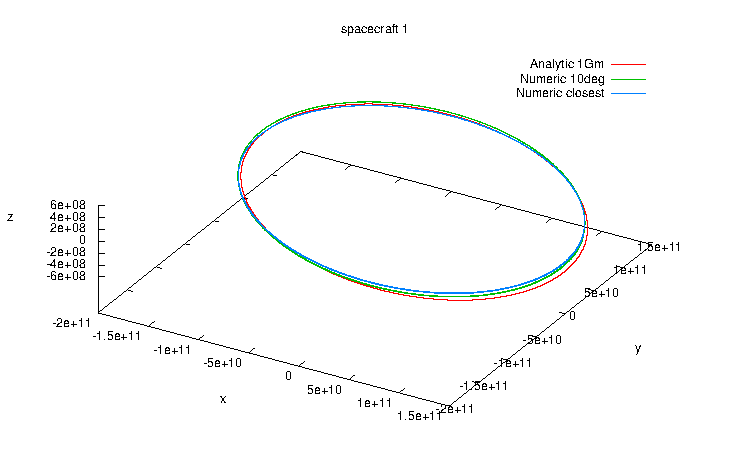
\includegraphics[scale=0.5,clip]{FigNoiseOrbSens/Orb_SC1_LISA-CLISA-10LISA.pdf}
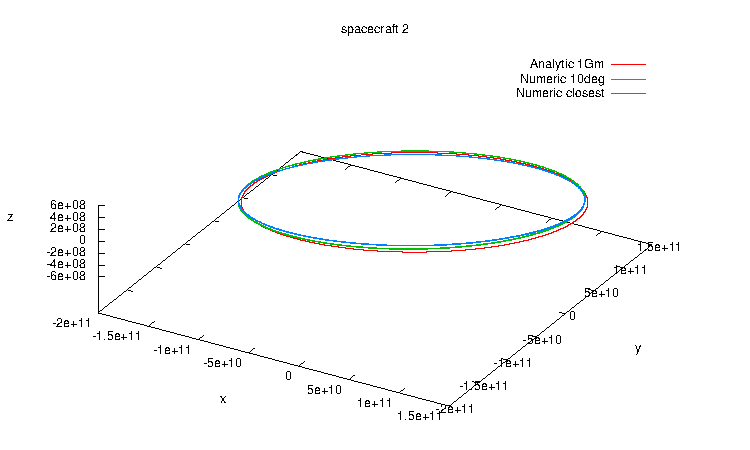
\includegraphics[scale=0.5,clip]{FigNoiseOrbSens/Orb_SC2_LISA-CLISA-10LISA.pdf}
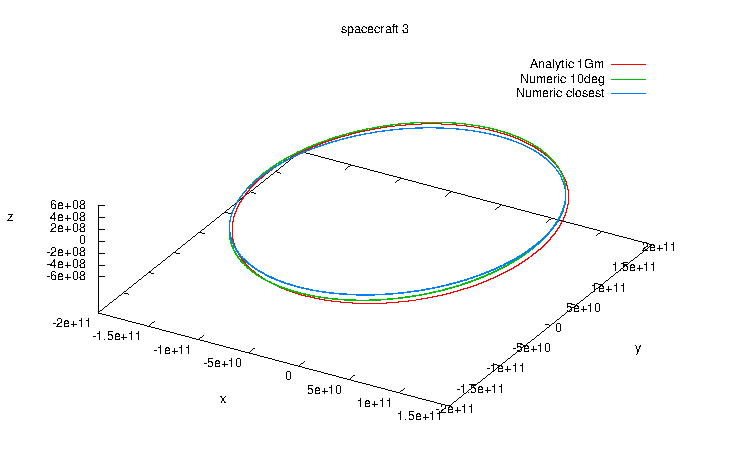
\includegraphics[scale=0.5,clip]{FigNoiseOrbSens/Orb_SC3_LISA-CLISA-10LISA.pdf} 
\end{center}
\caption{Orbits of the 3 spacecrafts.
\label{F:OrbSC} } 
\end{figure}

The main difference between this orbits is the time variation of the armlength as shown on the figure \ref{Arm-1_LISA-CLISA-10LISA}.
This is an important point for the technological design of the detector (Doppler effect, ...) and for the application of the Time Delay Interferometry which is the pre-data-analysis method for reducing the laser noise. 

\begin{figure}
\begin{center}
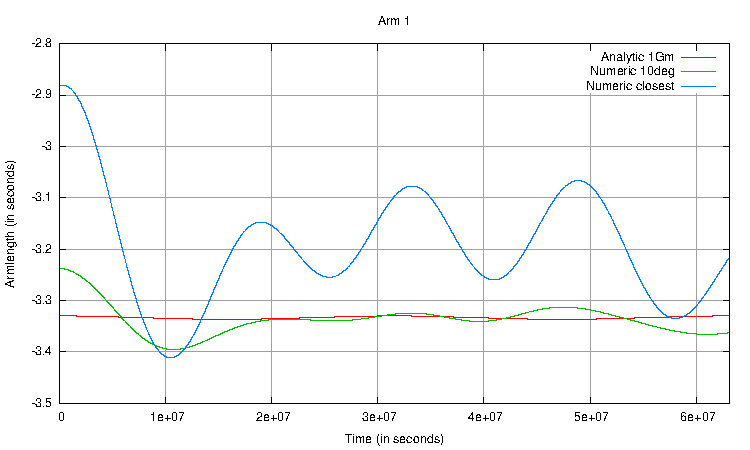
\includegraphics[scale=0.5,clip]{FigNoiseOrbSens/Arm-1_LISA-CLISA-10LISA.pdf}
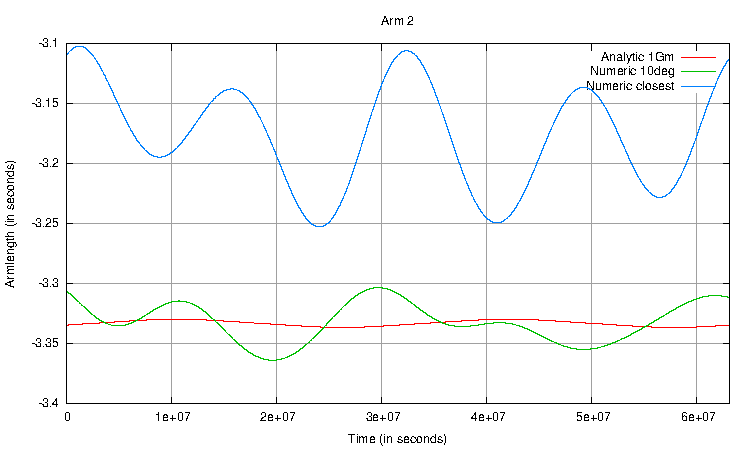
\includegraphics[scale=0.5,clip]{FigNoiseOrbSens/Arm-2_LISA-CLISA-10LISA.pdf}
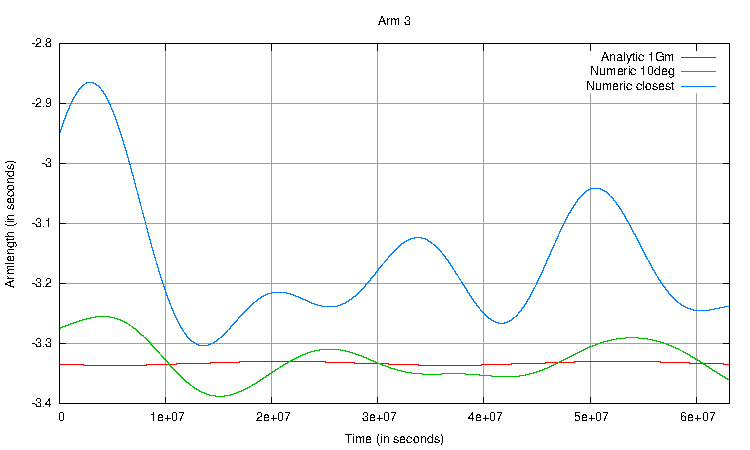
\includegraphics[scale=0.5,clip]{FigNoiseOrbSens/Arm-3_LISA-CLISA-10LISA.pdf} 
\end{center}
\caption{Time evolution of the 3 armlength during 2 years.
\label{F:ArmEvol} } 
\end{figure}

\subsubsection{Halo around L1}
\label{SS:Inst:Orb:HL1}

We test another kind of orbits : the Halo around Lagrange point L1.
This orbits are the results of numerical simulation done by Vitali Mueller (AEI-Hannover).
It's a mother/daughter configuration : there are only 4 links (2 arms).
The figure \ref{F:HL1Orb} shows the orbits and the figure \ref{F:HL1Arm} shows the armlength evolution.

\begin{figure}
\begin{center}
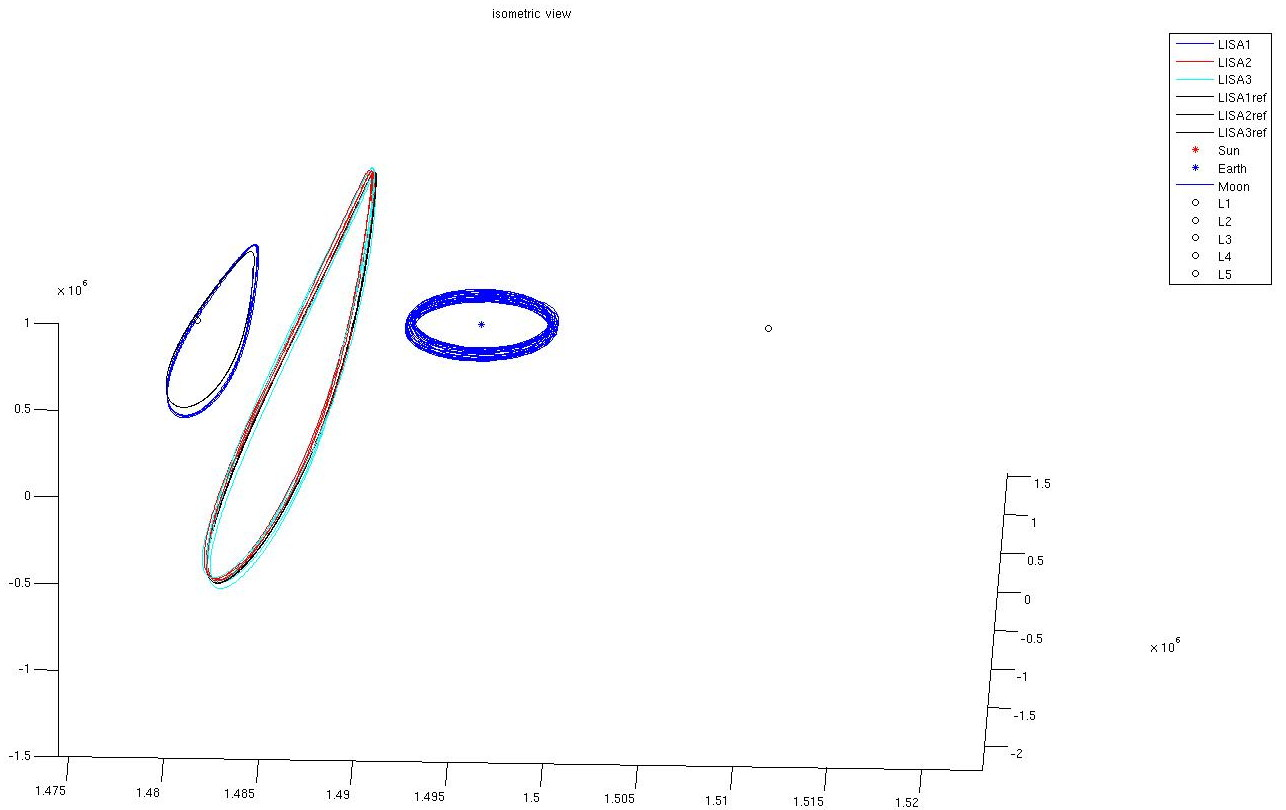
\includegraphics[width=\textwidth, clip]{FigNoiseOrbSens/HL1isometric.jpg}
\end{center}
\caption{Orbits of spacecraft for the Halo around L1 configuration.
\label{F:HL1Orb} } 
\end{figure}

\begin{figure}
\begin{center}
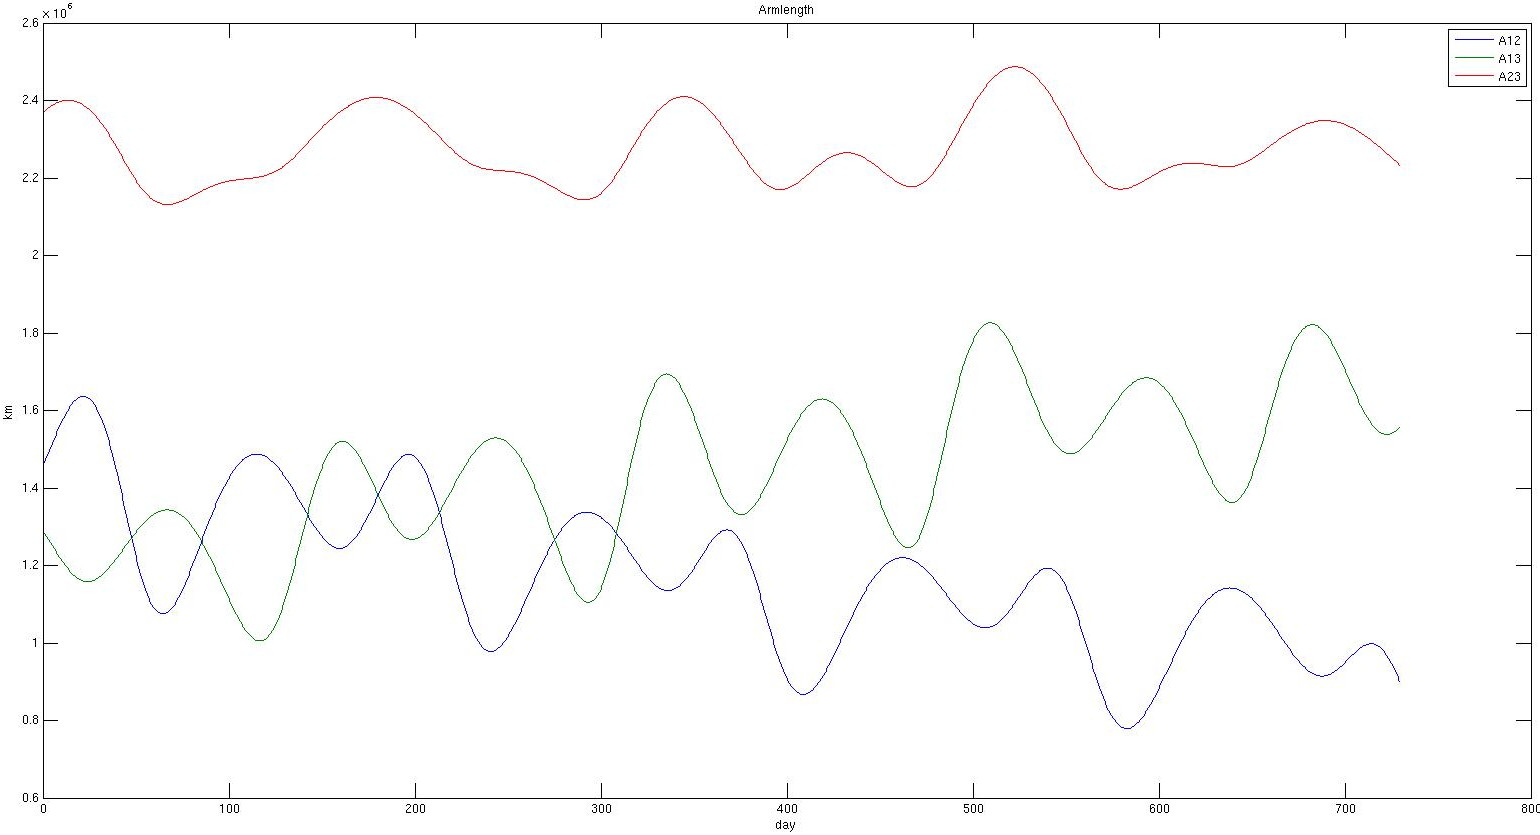
\includegraphics[width=\textwidth, clip]{FigNoiseOrbSens/HL1armlength.jpg}
\end{center}
\caption{Evolution of armlength for the Halo around L1 configuration.
\label{F:HL1Arm} } 
\end{figure}



The main spacecraft (mother) is on a close orbit around L1 and the 2 daughters are on a distant orbits separated in phase by  $\pi$.
The angle between the 2 arms is around 120$^o$. The armlengths evolve between 1 and 1.6 million km.




\subsection{Noise power spectral density (PSD) }
\label{SS:Inst:PSD}


\subsubsection{Analytical model}
\label{SSS:Inst:PSD:Ana}

The  analytic formulation of the Power Spectral Density of TDI X can be approximated by (usual approximation used in LISA) : 
\begin{equation}
S^X_{n, {\delta \nu \over \nu}}(f) = 16 * \sin^2(\phi_L(f))  \left(  S_{SN, {\delta \nu \over \nu}}(f) + S_{OMN, {\delta \nu \over \nu}}(f) + \left( 3 + \cos(2 \phi_L(f) ) \right) S_{acc, {\delta \nu \over \nu}}(f) \right) 
\label{PSDXNoiseLISA}
\end{equation}
with $ \phi_L(f) =  2 \pi f L/c $

\begin{figure}[htbp]
\begin{center}
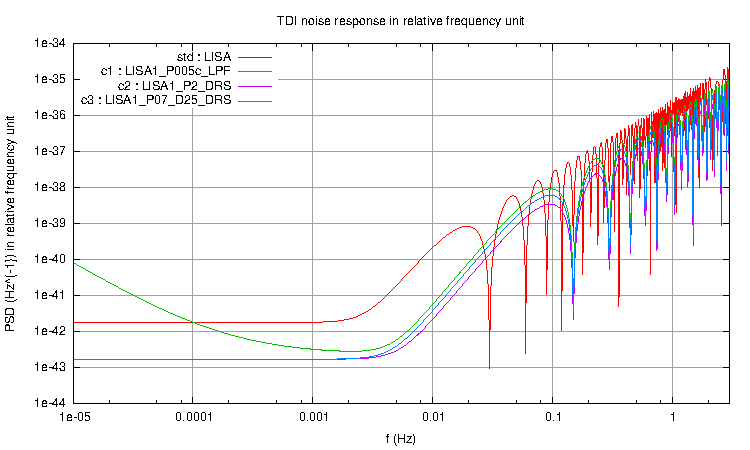
\includegraphics[width=0.9\textwidth]{FigNoiseOrbSens/PSD-Noise_std-c1-c2-c3}
\caption{Comparison of power spectral density of noises' response for  standard LISA, configurations 3a, 4a and 5a}
\label{F:PSDNoiseCompC3C4C5}
\end{center}
\end{figure}


\begin{figure}[htbp]
\begin{center}
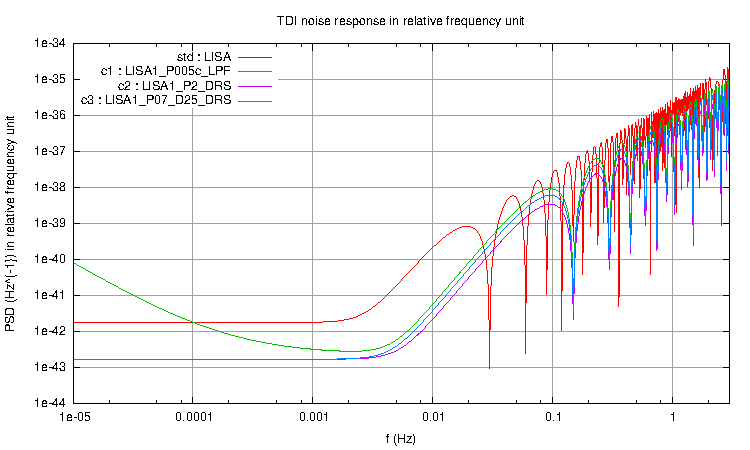
\includegraphics[width=0.9\textwidth]{FigNoiseOrbSens/PSD-Noise_std-c1-c2-c3}
\caption{Comparison of power spectral density of noises' response for standard LISA, configurations 1c, 2 and 3}
\label{F:PSDNoiseCompC1C2C3}
\end{center}
\end{figure}



\subsubsection{Simulation}
\label{SSS:Inst:PSD:Sim}






\subsection{Sensitivity}
\label{SS:Inst:Sensitivty}

\subsubsection{Analytical model}
\label{SSS:Inst:PSD:Ana}

(Very) approximative analytic formulation (based on LISA science requirements document (2010)) : 

The transfert function is 
\begin{equation}
T(f) = \sqrt{ 1 + \left( { f \over (0.41 \left({c \over 2 L} \right) )} \right)^2 }
\label{TransfertLISA}
\end{equation}

Sensitivity formulation :
\begin{equation}
\sqrt{S^{X}_h}(f) = \sqrt{5}  {2 \over \sqrt{3}} T(f)  { \sqrt{ 4 S_{acc} + S_{SN} + S_{omn} } \over L}
\label{AppSensXLISA}
\end{equation}


\begin{figure}[htbp]
\begin{center}
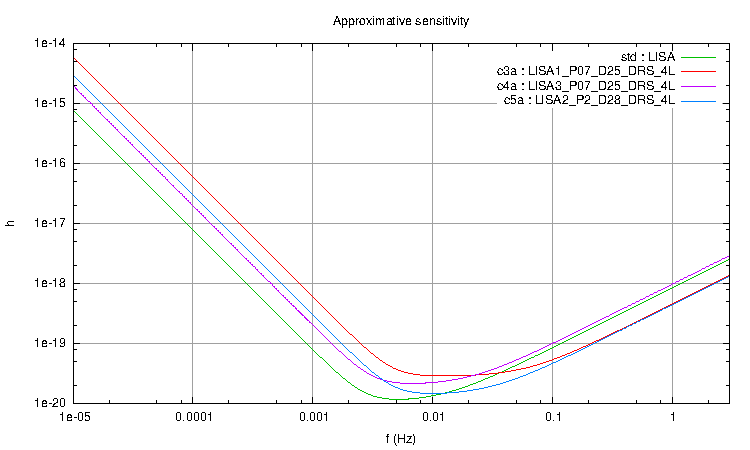
\includegraphics[width=0.9\textwidth]{FigNoiseOrbSens/Sensitivity_std-c3-c4-c5}
\caption{Comparison of sensitivity (SNR=1, "instantaneous") for standard LISA, configurations 3a, 4a and 5a}
\label{F:SensCompC3C4C5}
\end{center}
\end{figure}


\begin{figure}[htbp]
\begin{center}
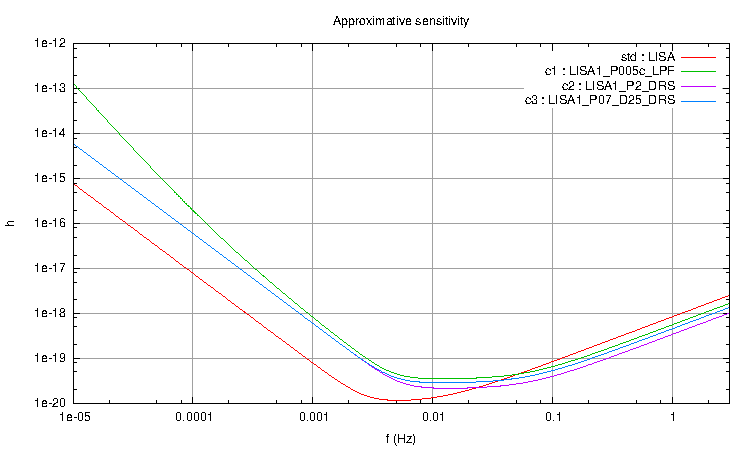
\includegraphics[width=0.9\textwidth]{FigNoiseOrbSens/Sensitivity_std-c1-c2-c3}
\caption{Comparison of sensitivity (SNR=1, "instantaneous") for standard LISA, configurations 1c, 2 and 3}
\label{F:SensCompC1C2C3}
\end{center}
\end{figure}


\subsubsection{Simulation}
\label{SSS:Inst:PSD:Sim}



%%%%%%%%%%%%%%%%%%%%%%%%%%%%%%%%%%%%%
%                                                 Galactic binaries                                                 %
%%%%%%%%%%%%%%%%%%%%%%%%%%%%%%%%%%%%%

\section{ Galactic binaries : confusion noise and galactic binaries}
\label{S:GalBin}
{ \it \small ('section captain' : Tyson Littenberg)}












%%%%%%%%%%%%%%%%%%%%%%%%%%%%%%%%%%%%%
%                                     Massive Black Hole binaries                                        %
%%%%%%%%%%%%%%%%%%%%%%%%%%%%%%%%%%%%%

\section{ Massive Black Hole binaries}
\label{S:MBHb}
{ \it ('section captain' : Alberto Sesana)}















%%%%%%%%%%%%%%%     MBHb : Parameter estimation
\subsection{Parameter estimation}
\label{SS:MBHbPE}
{\it ('section captains' : Neil Cornish \& Emanuele Berti) }




\subsubsection{PhenomC results from AEI {(S. Babak, A. Petiteau, A. Sesana, F. Ohme, E. Robinson)}}
\label{SSS:MBHbPEPhenomAEI}
We use PhenomC waveforms described in \cite{sm10}. Waveforms include merger and ringdown and assume aligned spins. Given the latter assumption, we apply them to efficient accretion models (SE, LE) only. Moreover, since the waveforms can not handle too extreme cases, we lower the maximal spin limit to 0.98, and considered only sources with mass ratio larger than $q=M_2/M_1=0.05$, thus loosing 10-20\% of the sources (depending on the MBH population model) in our analysis.

We consider a threshold SNR$=6$ for detection, and SNR$=10$ for trustworthy parameter estimations. We show results for detectors LISA, C4, C5, C2, C3 and C5,  assuming a single Michelson interferometer. 


Figures \ref{Hist_SE_LISAC2C4C5} and \ref{Hist_LE_LISAC2C4C5} show histograms of parameter estimation accuracy for the ten realizations of model SE and LE respectively with LISA, C2, C4 and C5; only sources with SNR$>10$ are included. 

The median parameter estimation accuracy with LISA, C2, C4 and C5 as a function of redshift is shown in figures \ref{MedianSNR_SE_LISAC2C4C5}-to-\ref{MedianSNR_LE_LISAC2C4C5}.

The median source SNR with LISA, C2, C4 and C5 as a function of redshift is shown in figures \ref{MedianSNR_SE_LISAC2C4C5}-to-\ref{MedianSNR_LE_LISAC2C4C5}.


\vspace{1cm}

For comparison we also add results comparing about C1, C2 and LISA and SNR for C3 : 

Figures \ref{LISA_mc_SNR}, \ref{C3_mc_SNR}, \ref{C2_mc_SNR} and \ref{C1_mc_SNR} show the performances of LISA, C2 and C1 respectively, assuming the SE MBH binary population model.



Figures \ref{Hist_SE_LISAC1C2} and \ref{Hist_LE_LISAC1C2} show histograms of parameter estimation accuracy for the ten realizations of model SE and LE respectively; only sources with SNR$>10$ are included. 
 

The median source SNR and parameter estimation accuracy as a function of redshift is shown in figures \ref{MedianErrs_SE_LISAC1C2}-to-\ref{MedianErrs_LE_LISAC1C2}.


%%%%%%%%%%%%%%%%  Histogram LISA, C2, C4 and C5  %%%%%%%%%%%%%%%%

\begin{figure}
\resizebox{\hsize}{!}{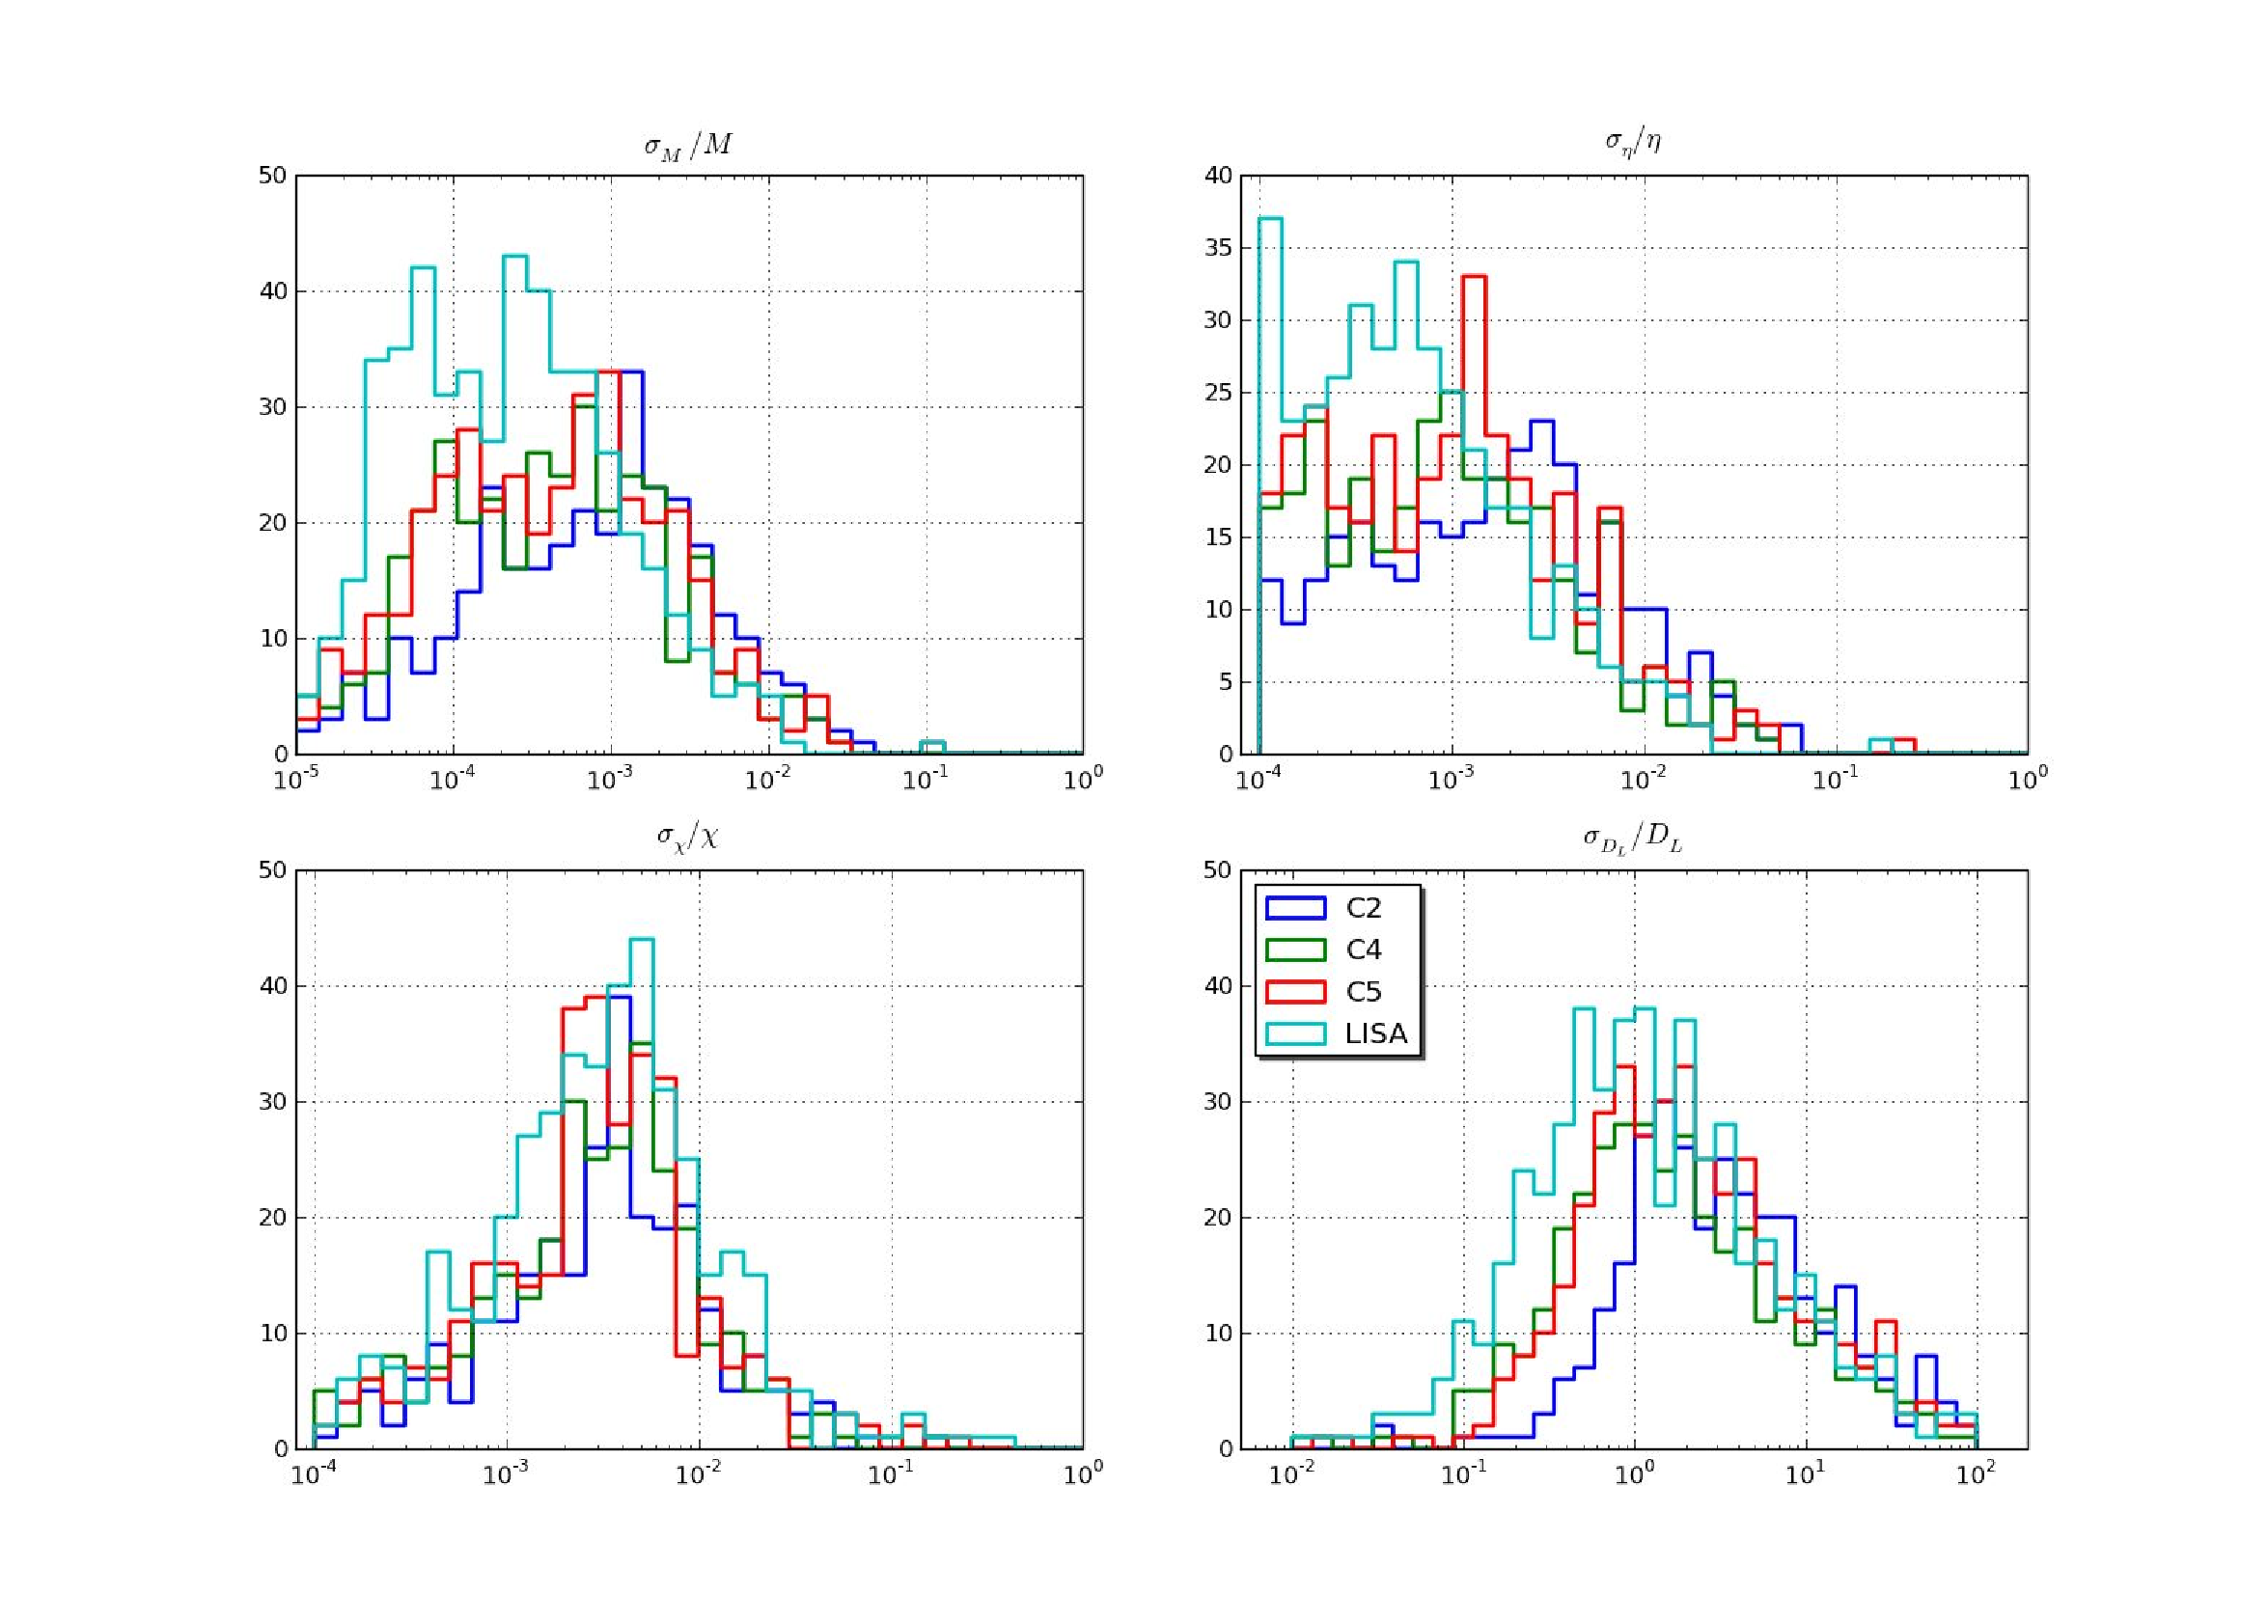
\includegraphics[scale=1,clip]{FigSMBHPhenomAEI/Hist_SE_LISAC2C4C5.eps}} 
\caption{1-$\sigma$ errors on source parameters: redshifted mass (upper left); symmetric mass ratio (upper right); spin parameter (lower left); luminosity distance (lower right). Histograms collect all the events in the SE catalogue (small seed), with SNR$>10$. Ligth blue histograms are for LISA, blue histograms are for C2, green histograms are for C4 and red histograms are for C5.
\label{Hist_SE_LISAC2C4C5} } 
\end{figure}

\begin{figure}
\resizebox{\hsize}{!}{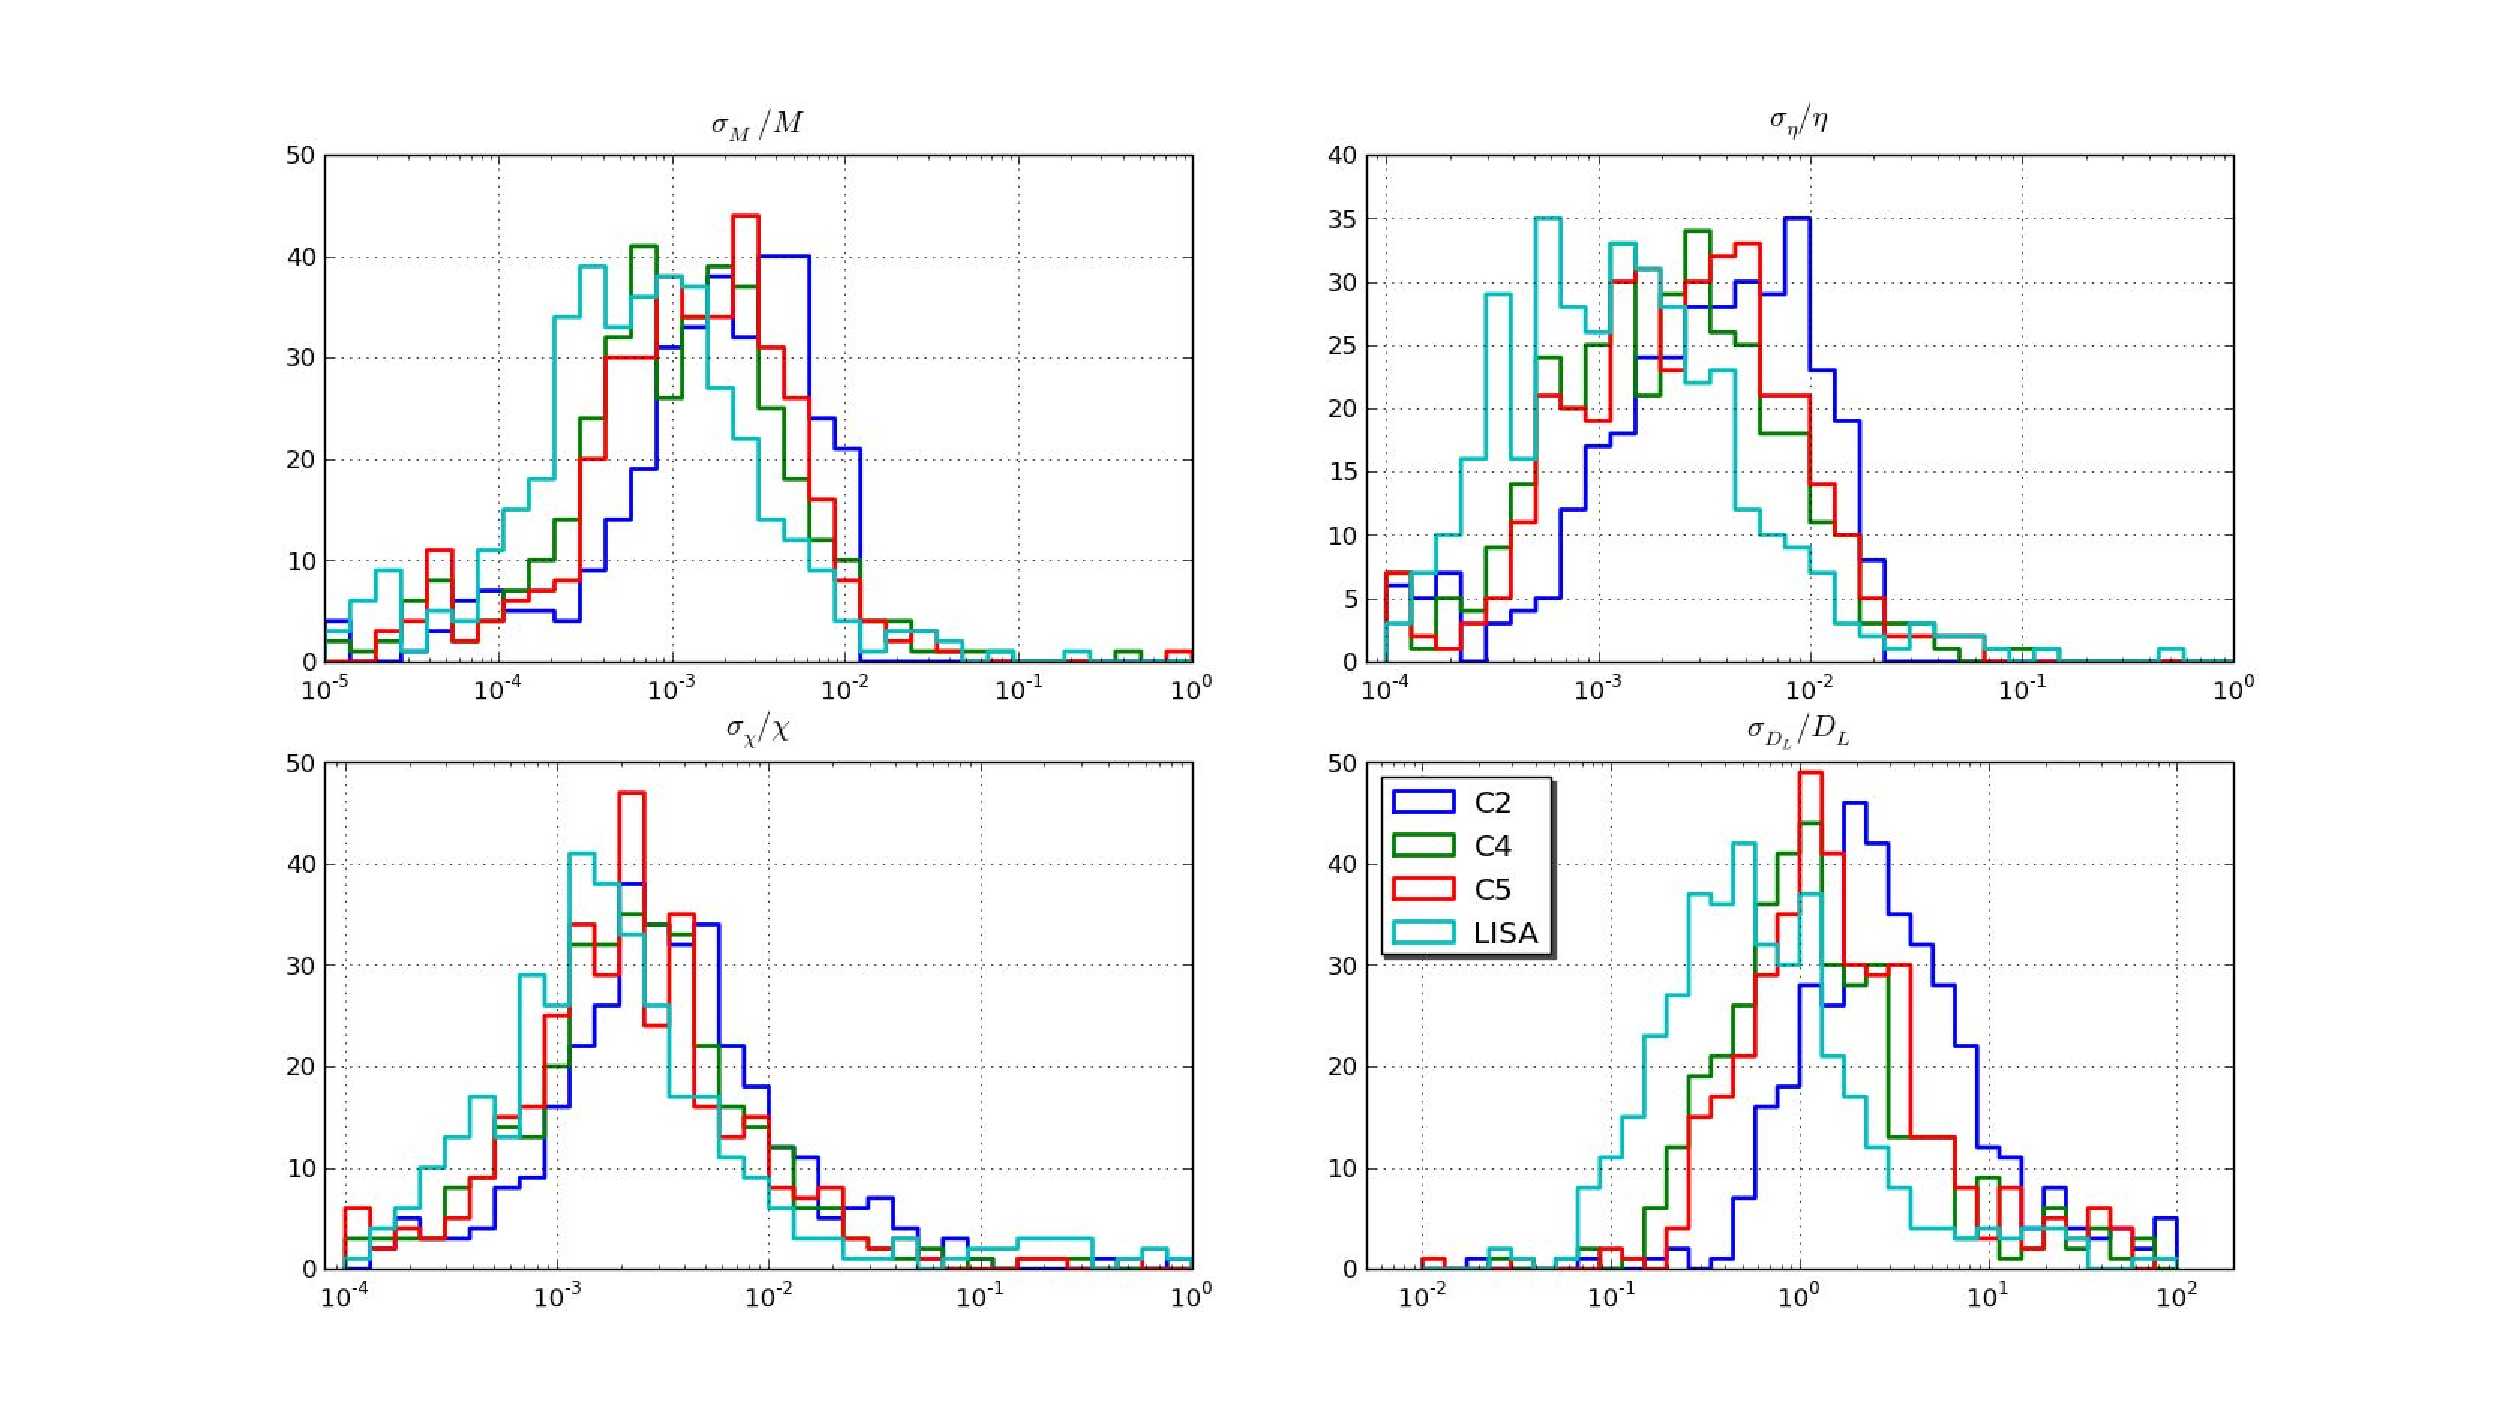
\includegraphics[scale=1,clip]{FigSMBHPhenomAEI/Hist_LE_LISAC2C4C5.eps}} 
\caption{1-$\sigma$ errors on source parameters. Similar as \ref{Hist_SE_LISAC2C4C5} with LE catalogue (large seed).
\label{Hist_LE_LISAC2C4C5} } 
\end{figure}


%%%%%%%%%%%%%%%%  Median errors LISA, C2, C4 and C5  %%%%%%%%%%%%%%%%

\begin{figure}
\resizebox{0.99\hsize}{!}{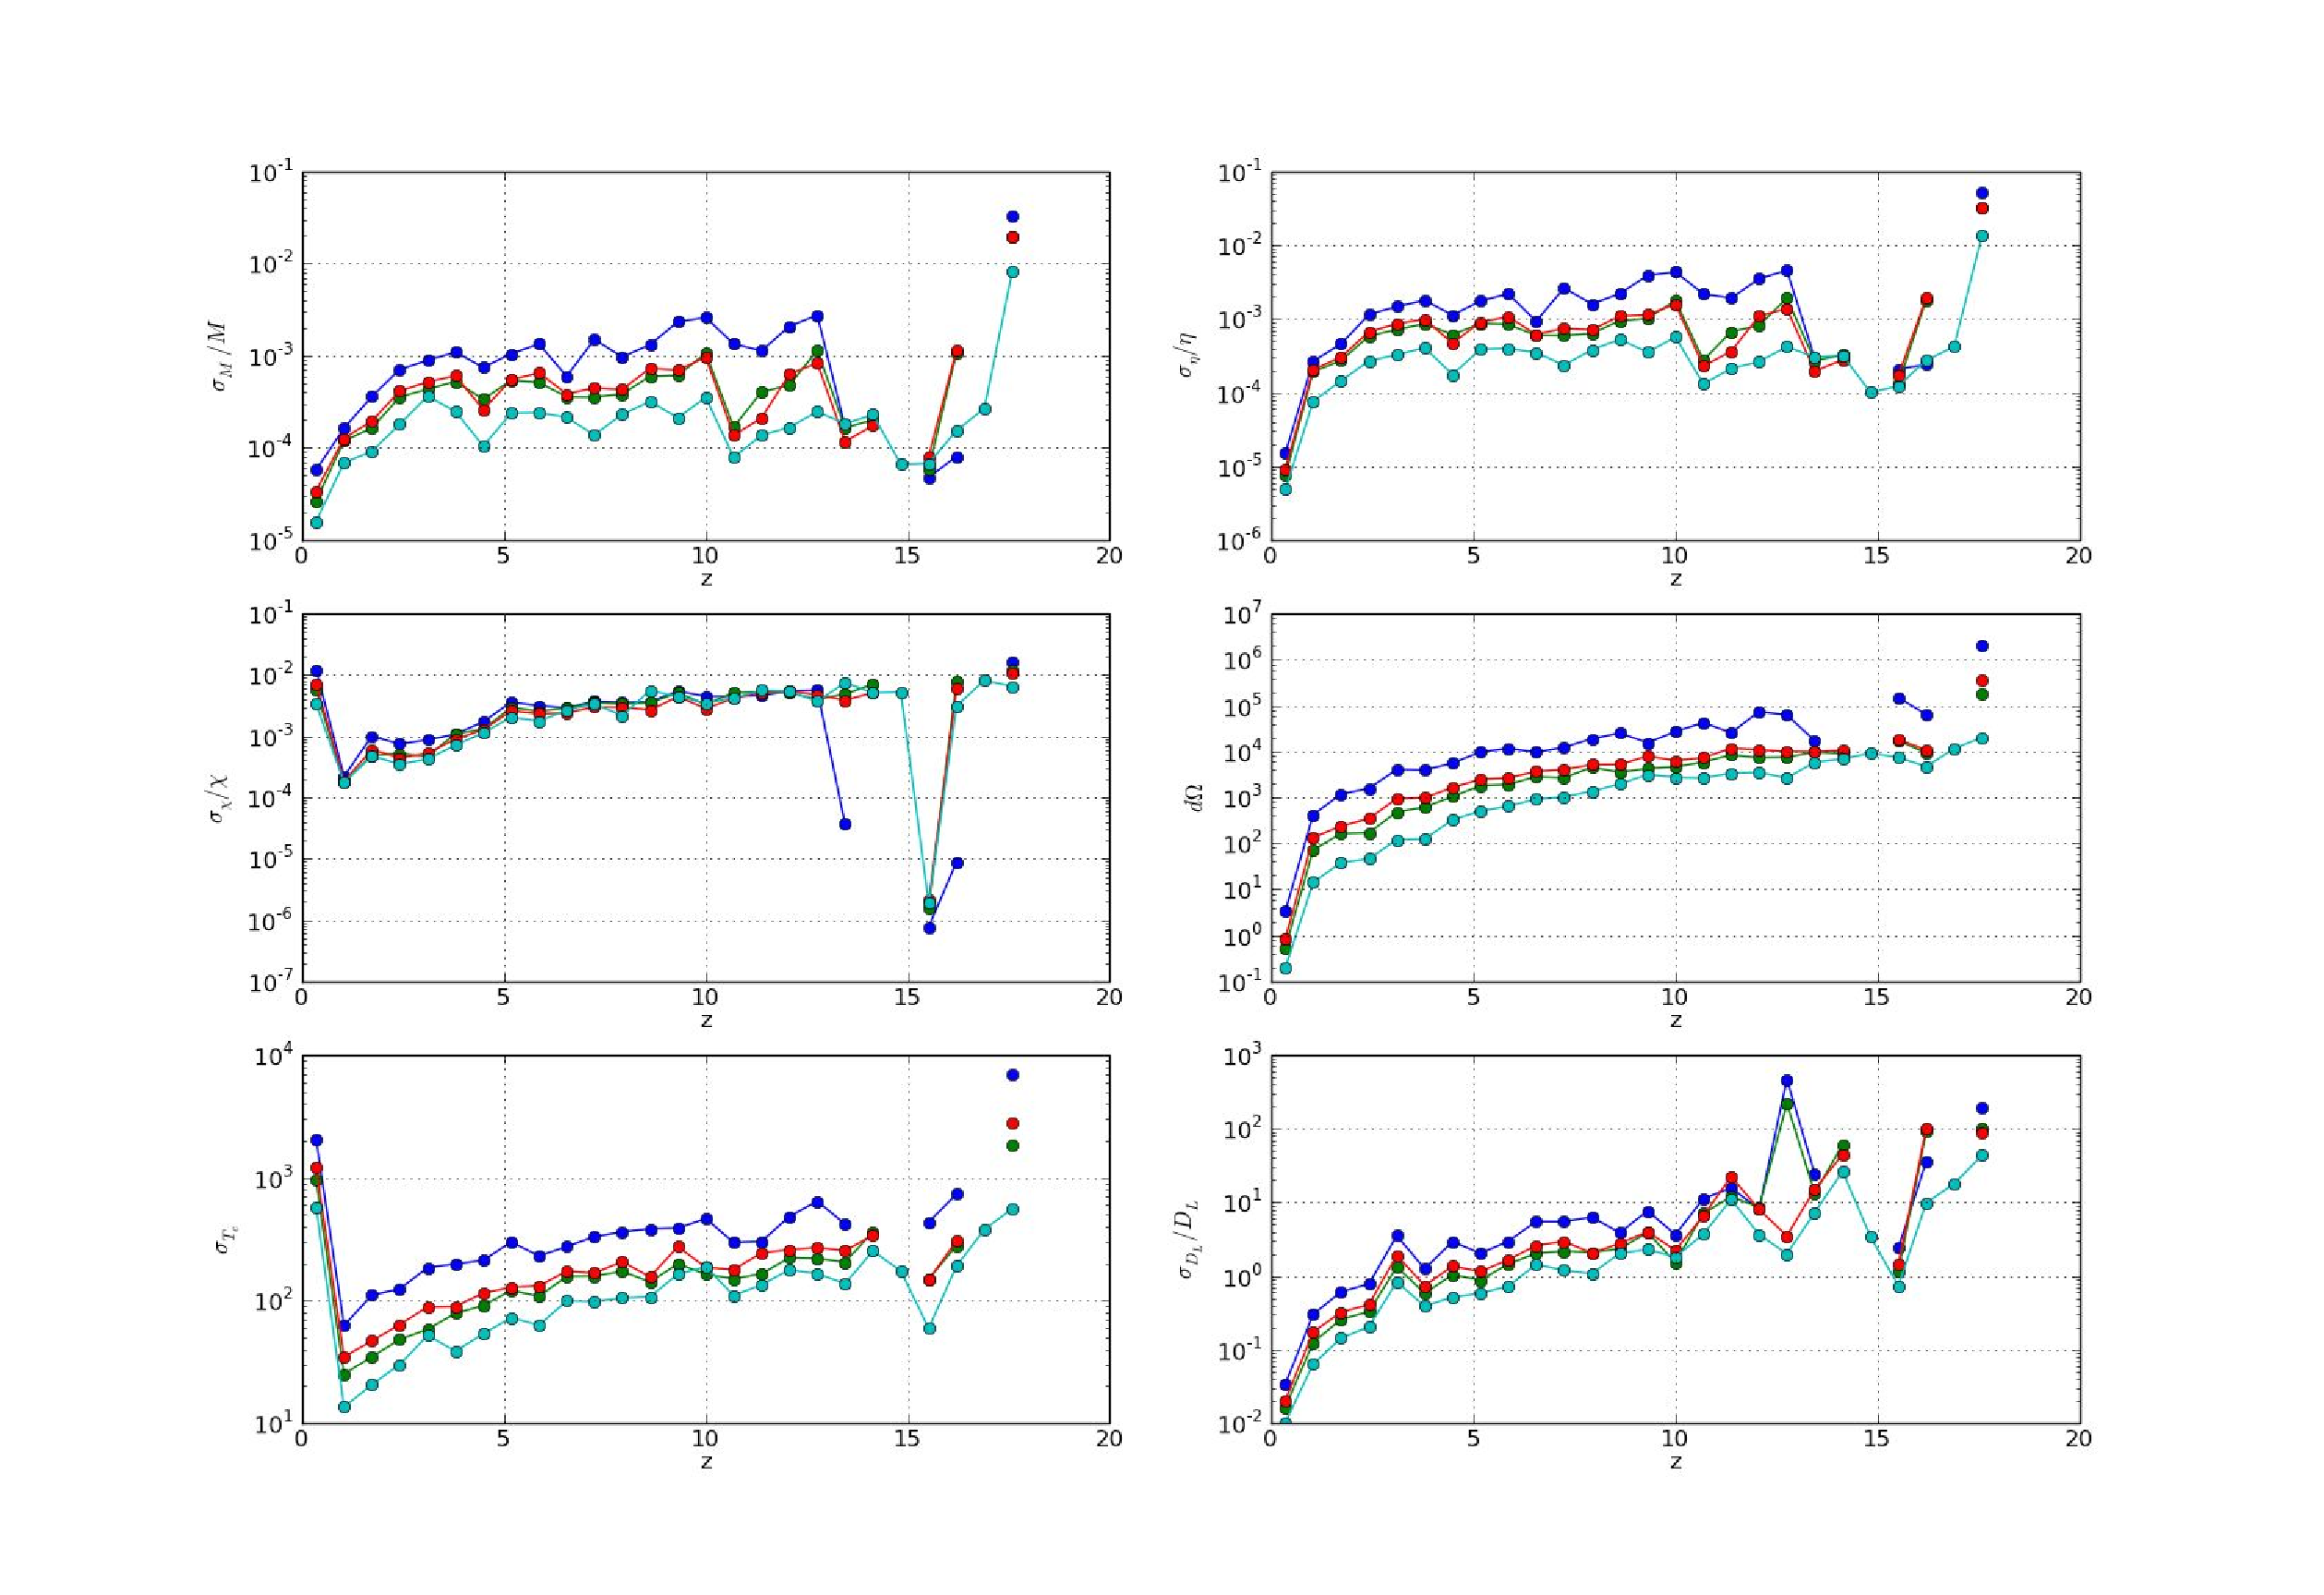
\includegraphics[scale=1,clip]{FigSMBHPhenomAEI/MedianErrs_SE_LISAC2C4C5.eps}} 
\caption{Median 1-$\sigma$ errors on the source parameters as a function of 
$z$: redshifted mass (upper left); symmetric mass ratio (upper right); spin parameter (middle left); sky location in deg$^2$ (middle right); coalescence time in seconds (lower left); luminosity distance (lower right). Colorstyle as in figure \ref{Hist_SE_LISAC2C4C5} : ligth blue histograms are for LISA, blue histograms are for C2, green histograms are for C4 and red histograms are for C5. Model SE (small seeds) is assumed.
\label{MedianErrs_SE_LISAC2C4C5} } 
\end{figure}

\begin{figure}
\resizebox{0.99\hsize}{!}{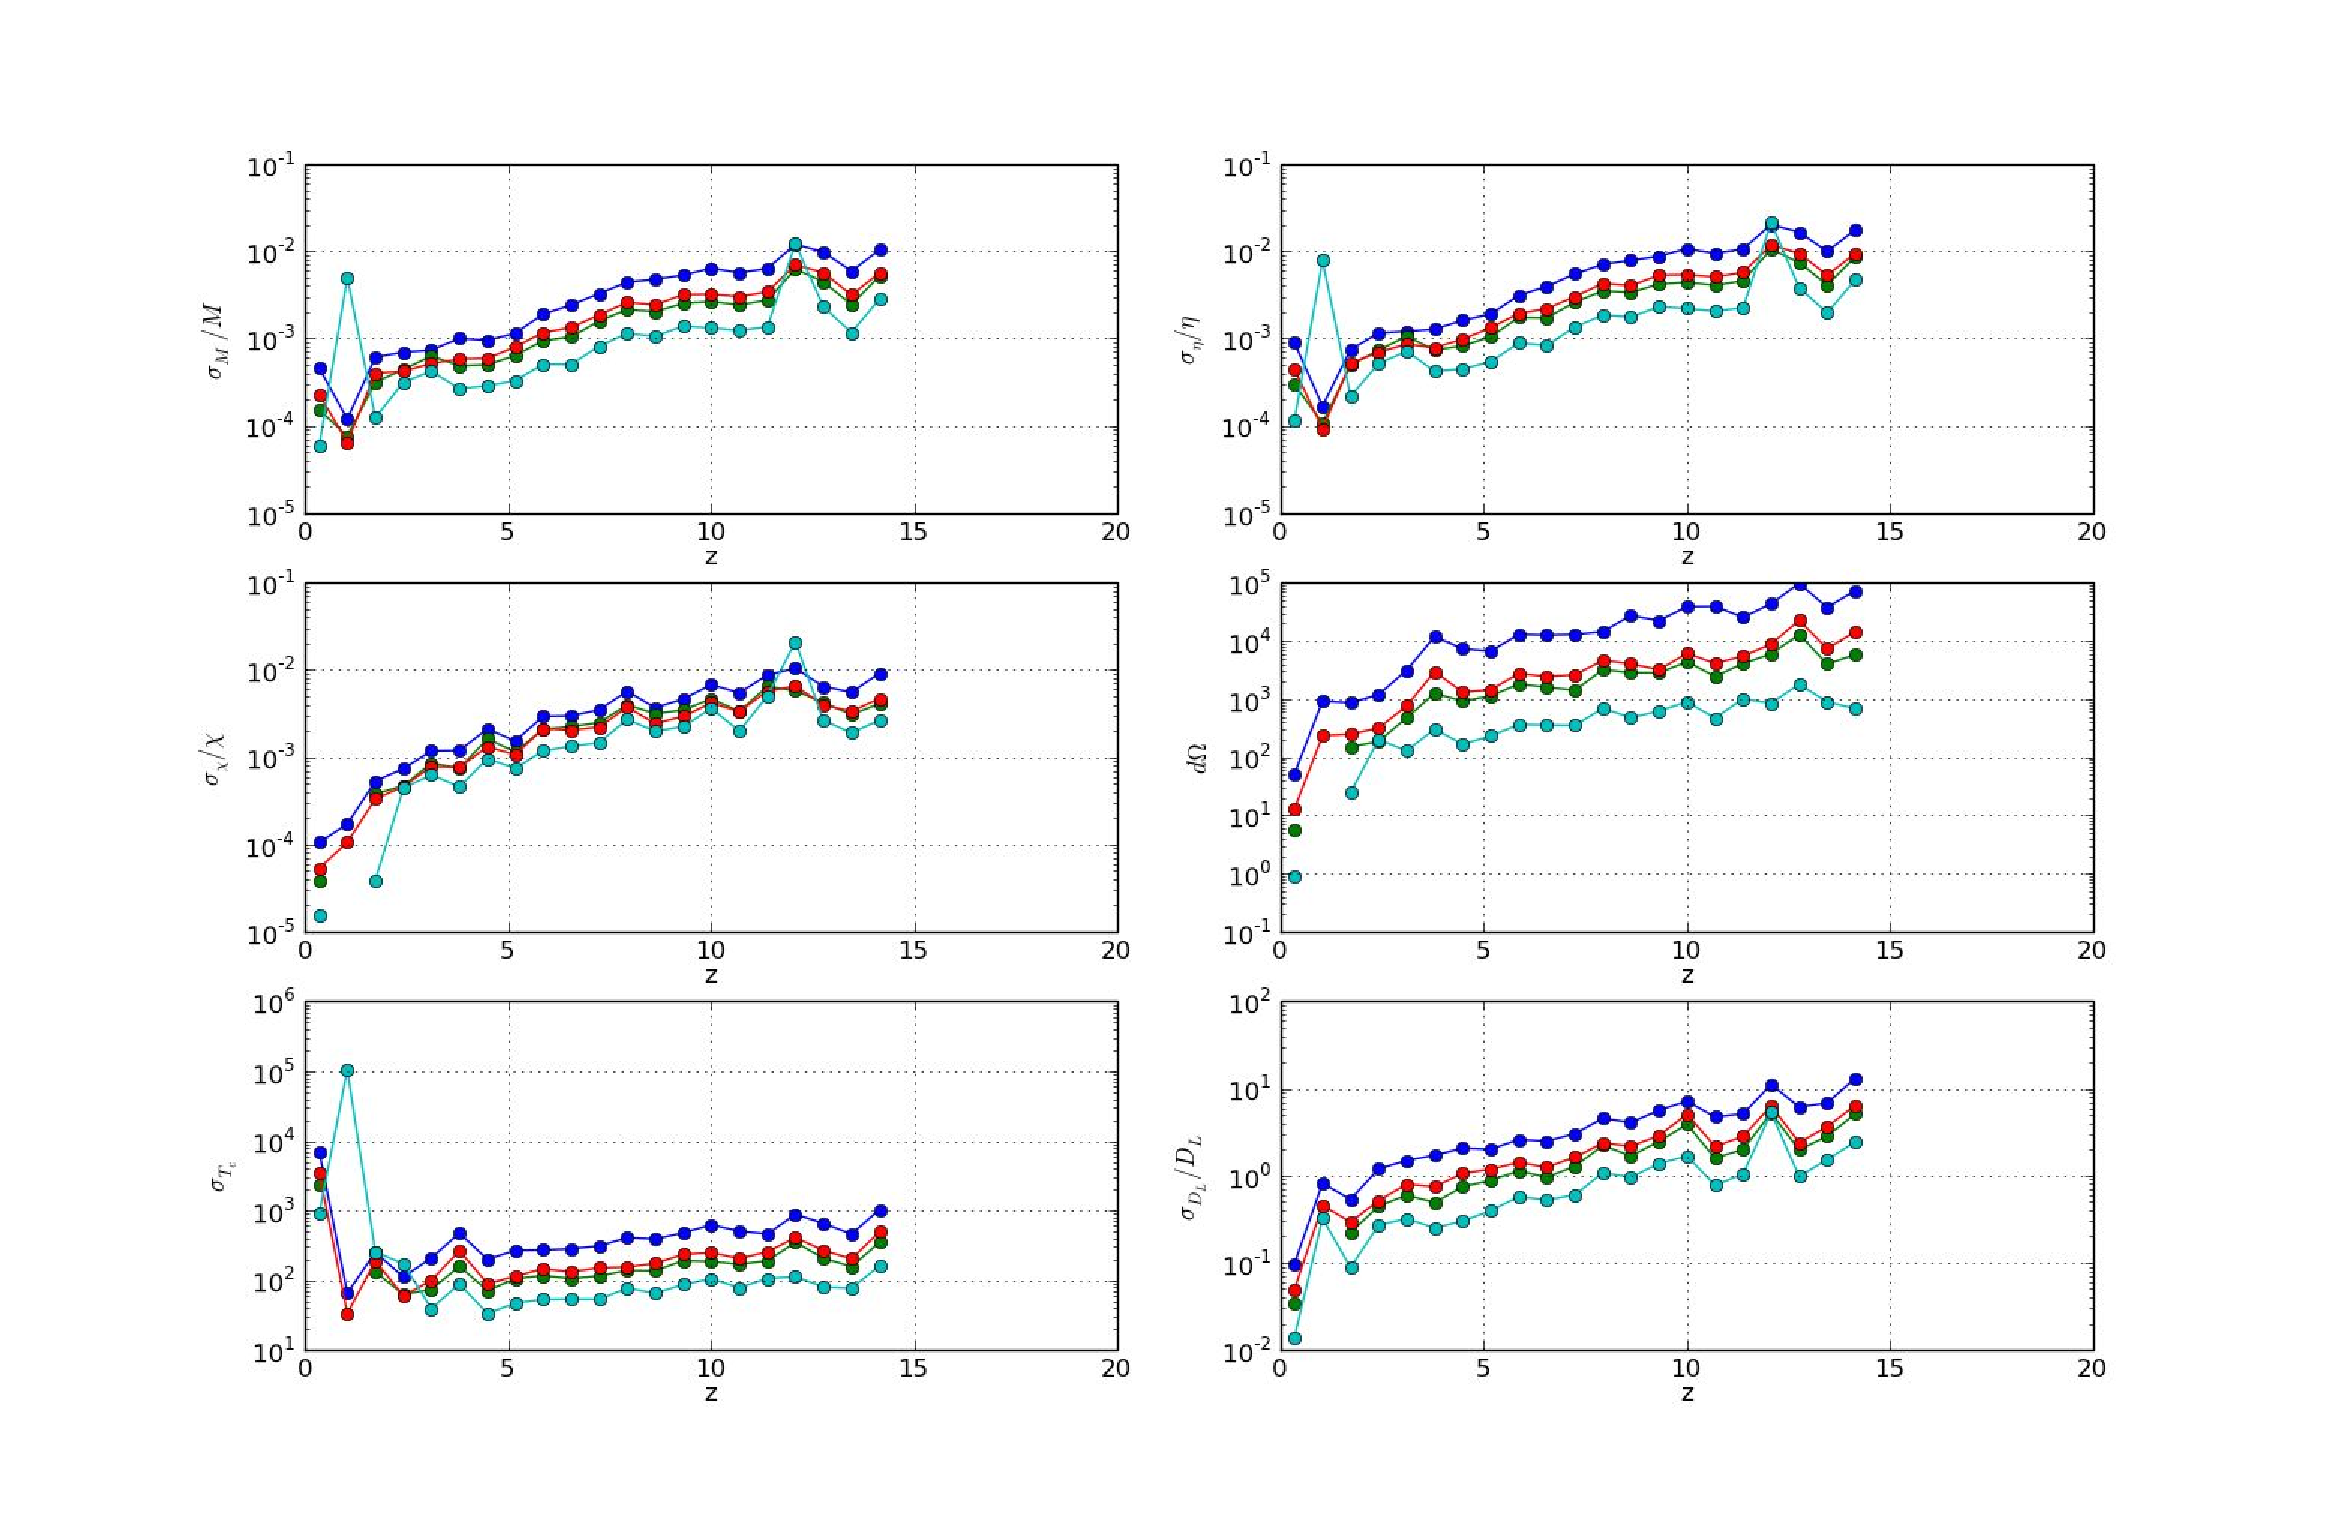
\includegraphics[scale=1,clip]{FigSMBHPhenomAEI/MedianErrs_LE_LISAC2C4C5.eps}} 
\caption{Same as figure \ref{MedianErrs_SE_LISAC2C4C5} but for the LE (large seed) catalogue.
\label{MedianErrs_LE_LISAC2C4C5} } 
\end{figure}


%%%%%%%%%%%%%%%%  Median SNR LISA, C2, C4 and C5  %%%%%%%%%%%%%%%%


\begin{figure}
\resizebox{0.95\hsize}{!}{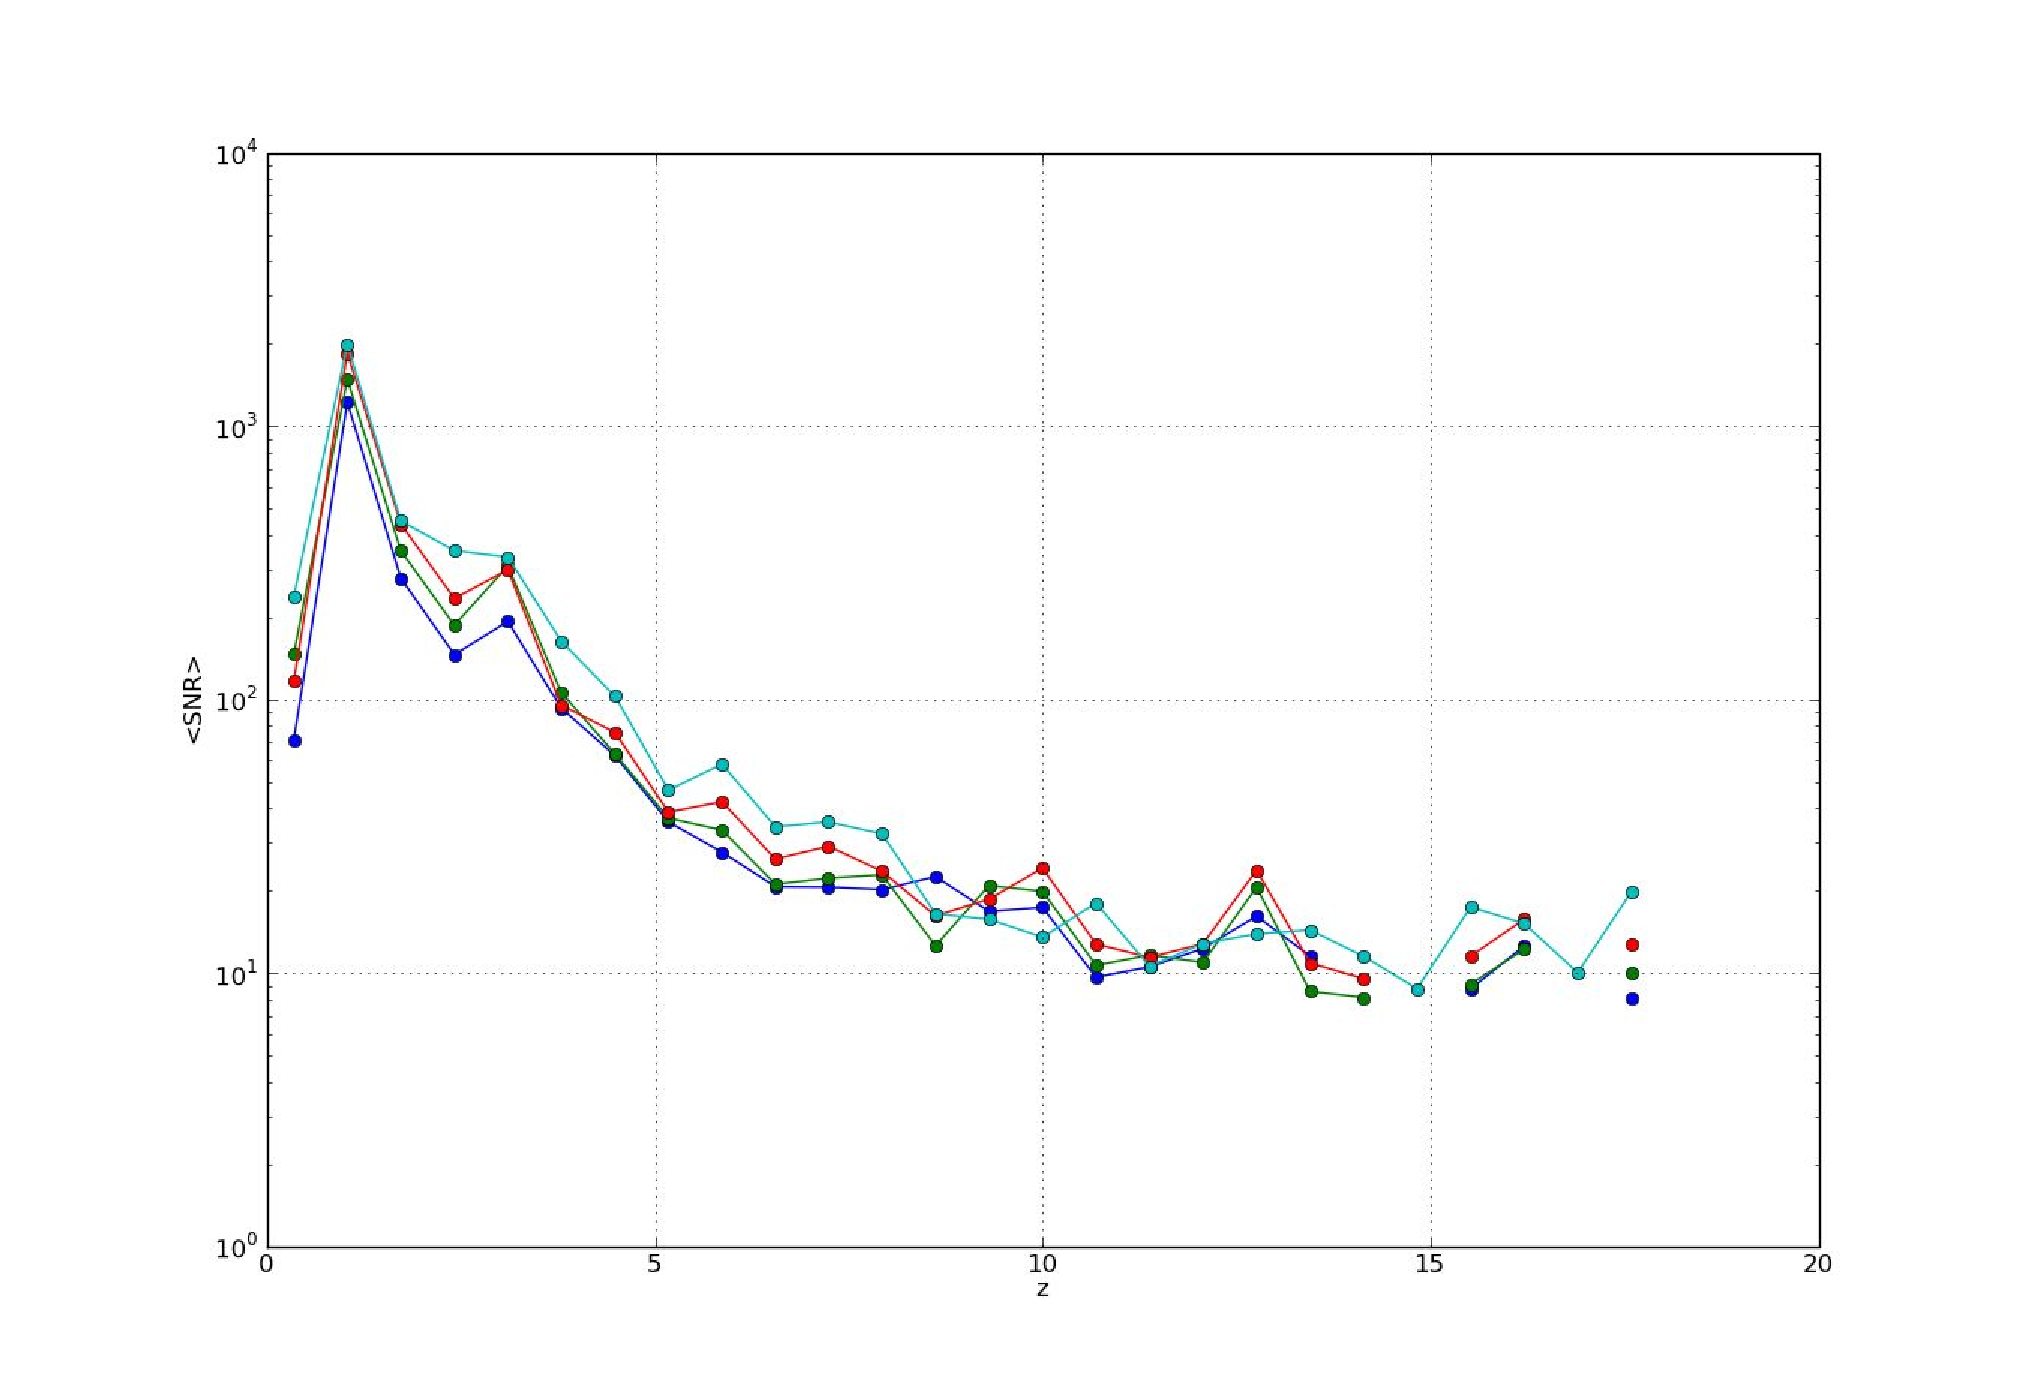
\includegraphics[scale=1,clip]{FigSMBHPhenomAEI/MedianSNR_SE_LISAC2C4C5.eps}} 
\caption{Median SNR s as a function of  $z$. Colorstyle as in figure \ref{Hist_SE_LISAC2C4C5} : ligth blue histograms are for LISA, blue histograms are for C2, green histograms are for C4 and red histograms are for C5. Model SE (small seeds) is assumed.
\label{MedianSNR_SE_LISAC2C4C5} } 
\end{figure}

\begin{figure}
\resizebox{0.95\hsize}{!}{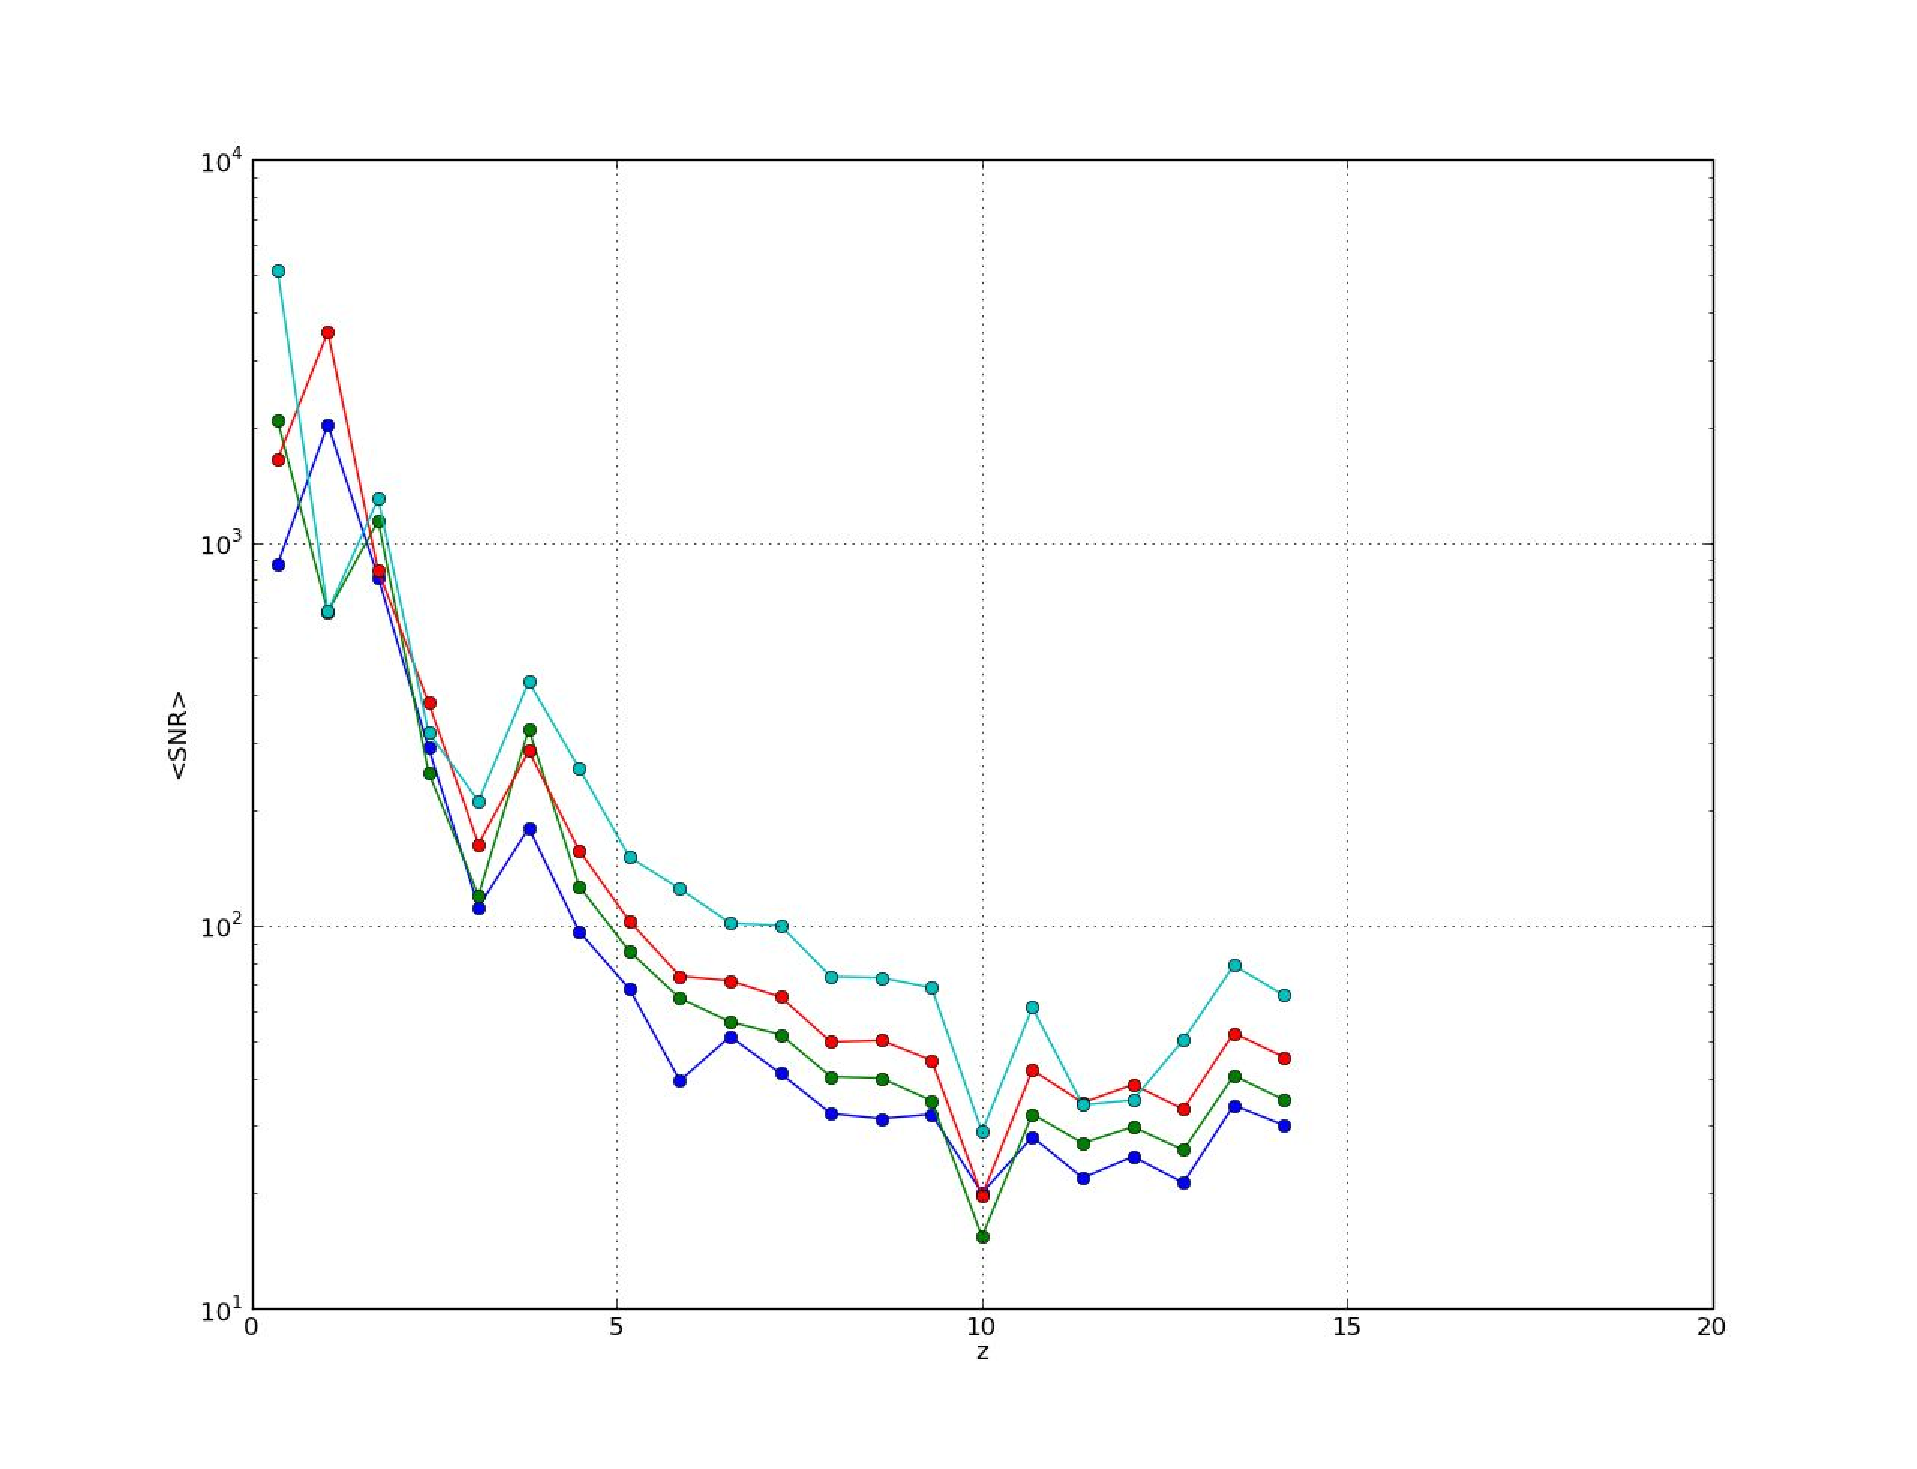
\includegraphics[scale=1,clip]{FigSMBHPhenomAEI/MedianSNR_LE_LISAC2C4C5.eps}} 
\caption{Same as figure \ref{MedianSNR_SE_LISAC2C4C5} but for the LE (large seed) catalogue.
\label{MedianSNR_LE_LISAC2C4C5} } 
\end{figure}


%%%%%%%%%%%%%%%%  SNR vs z LISA, C1 and C3  %%%%%%%%%%%%%%%%


\begin{figure}
\resizebox{\hsize}{!}{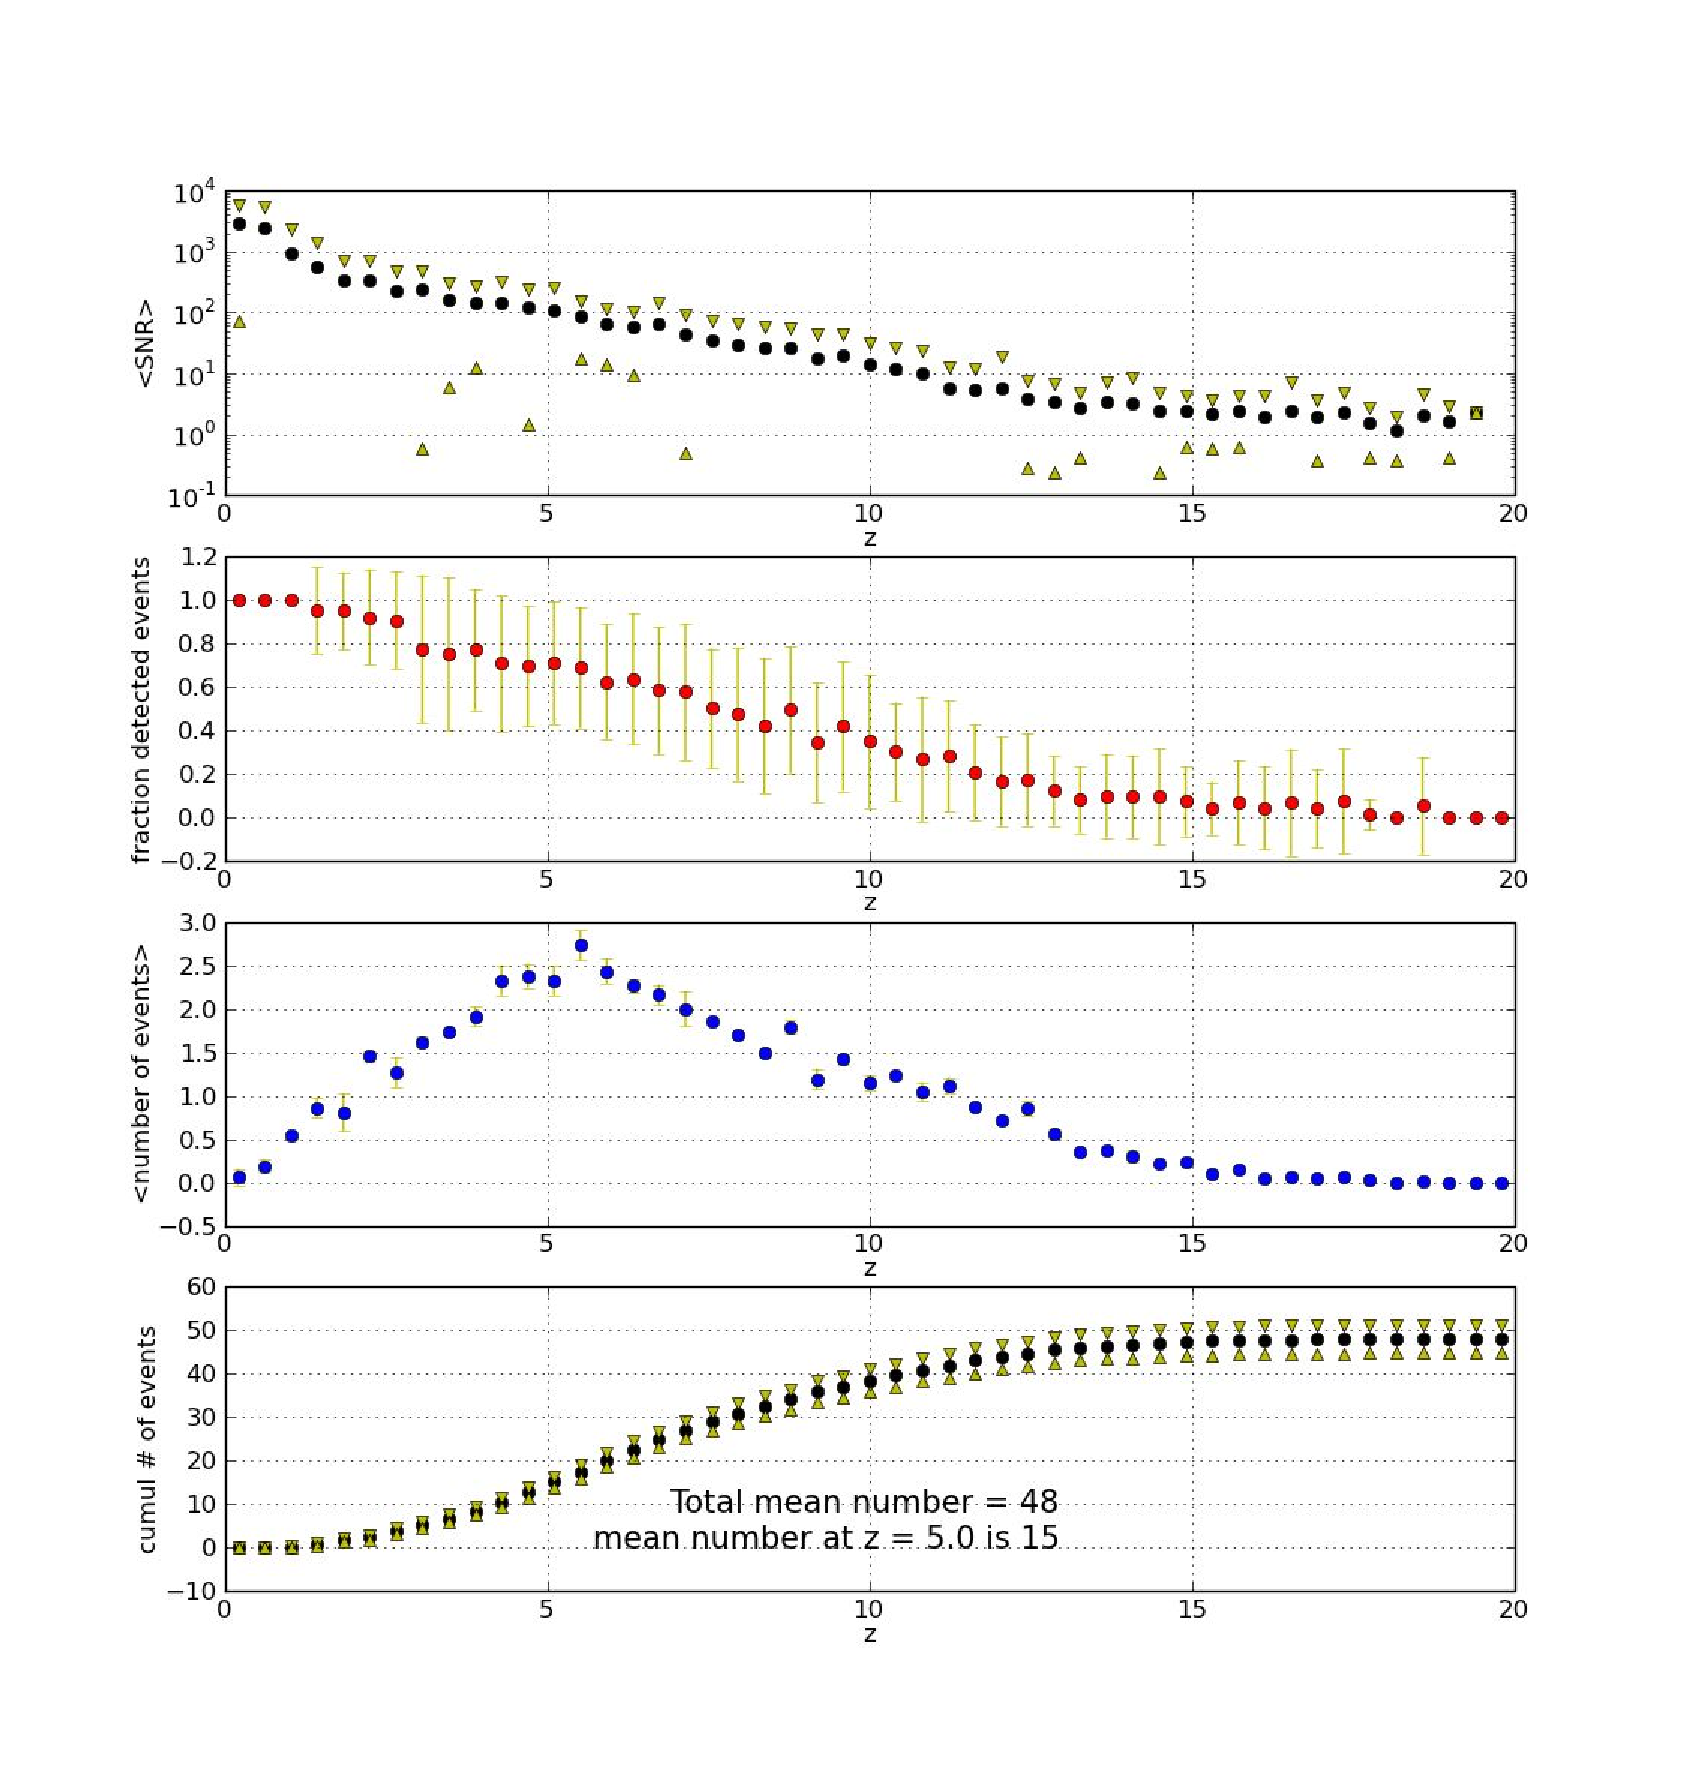
\includegraphics[scale=1,clip]{FigSMBHPhenomAEI/LISA_mc_SNRs.eps}} 
\caption{LISA performances as a function of redshift. From the top to the bottom we plot the average source SNR, the fraction of detectable sources (SNR$>6$), the mean number of detected sources, and the cumulative number of detected sources. Error bars are standard deviations; SE population model is assumed.
\label{LISA_mc_SNR} } 
\end{figure}


\begin{figure}
\resizebox{\hsize}{!}{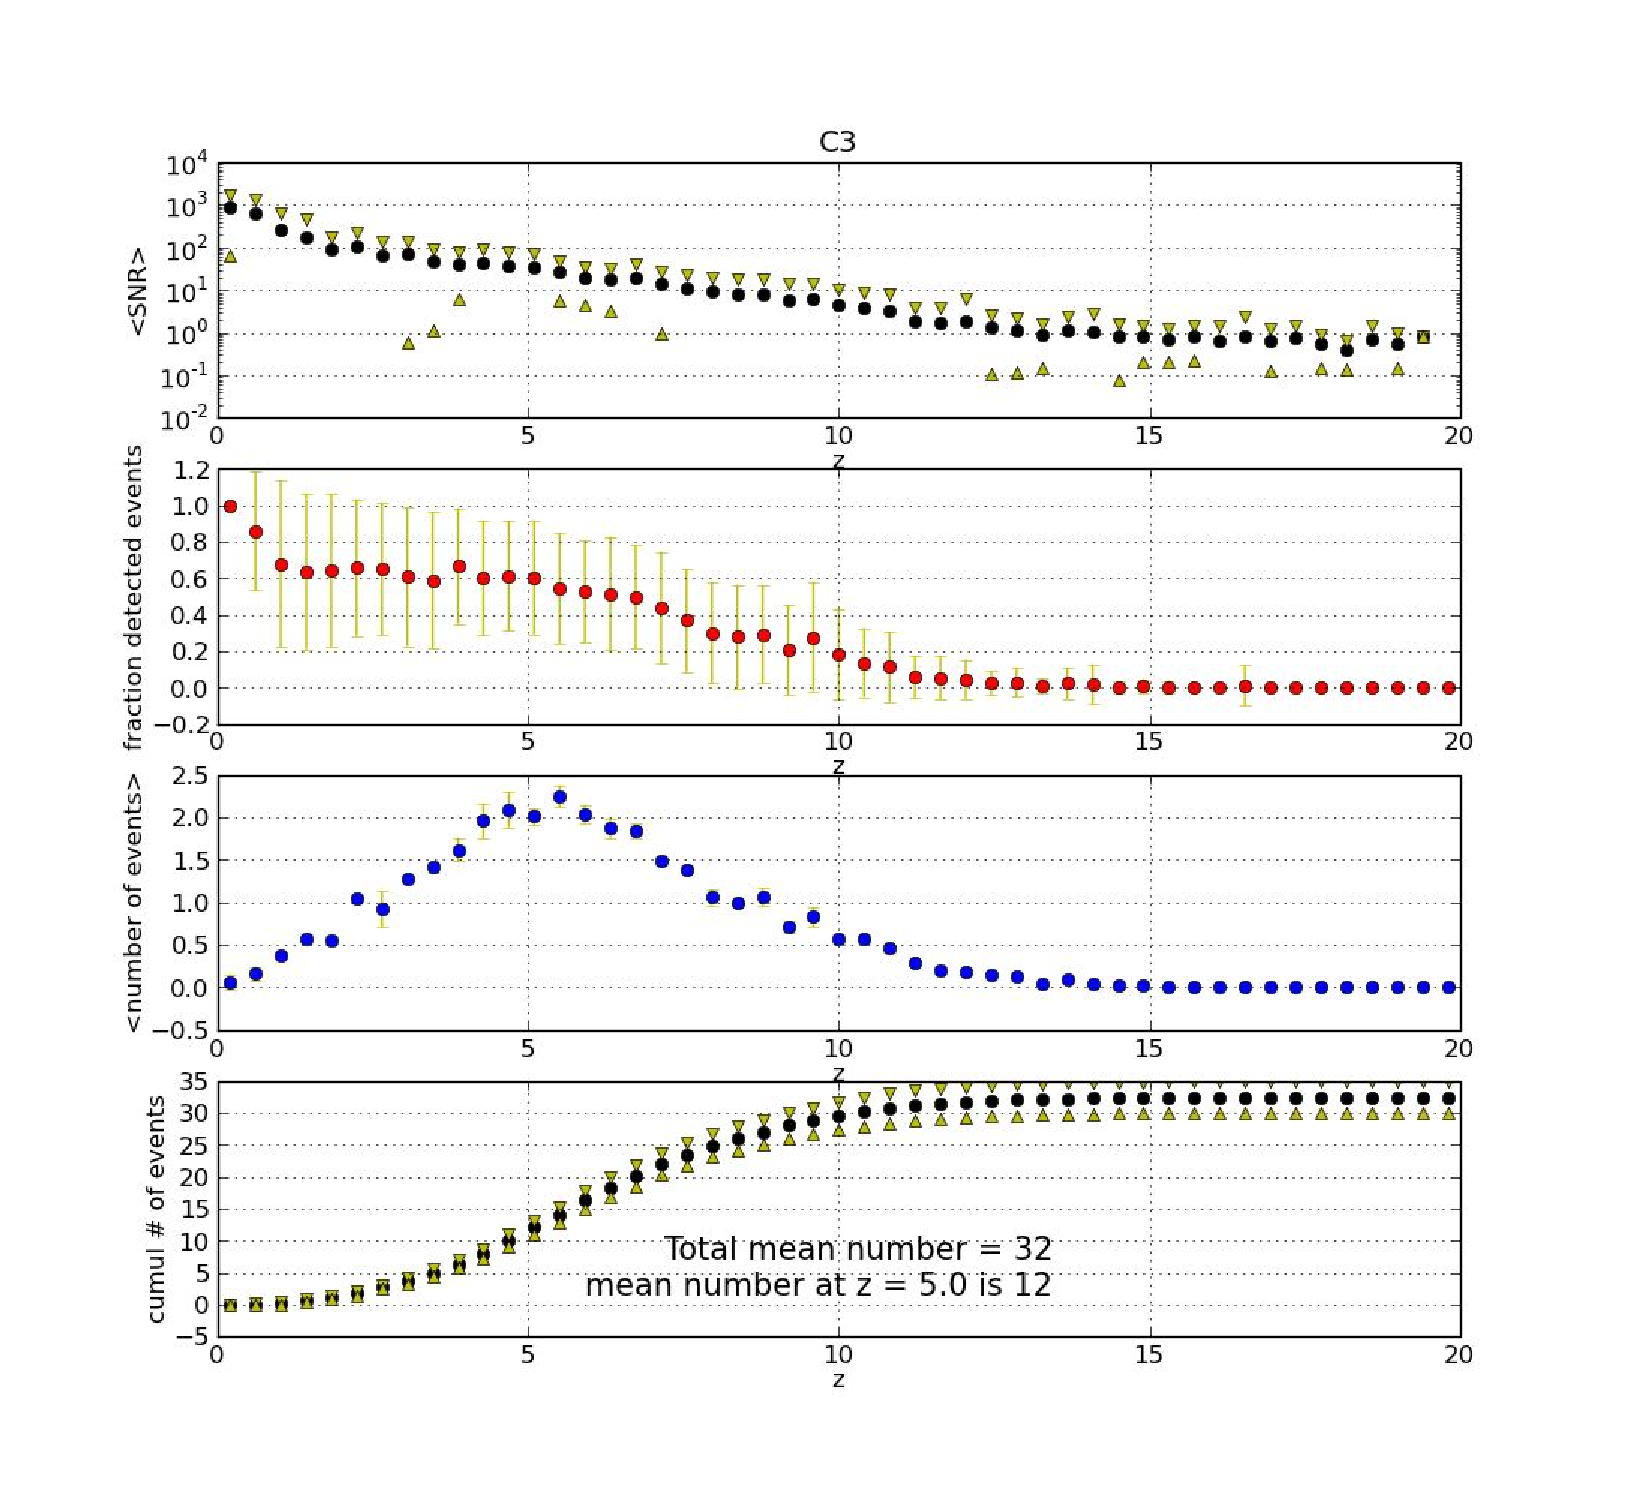
\includegraphics[scale=1,clip]{FigSMBHPhenomAEI/C3_mc_SNRs.eps}} 
\caption{Same as figure \ref{LISA_mc_SNR} but for C3.
\label{C3_mc_SNR} } 
\end{figure}


\begin{figure}
\resizebox{\hsize}{!}{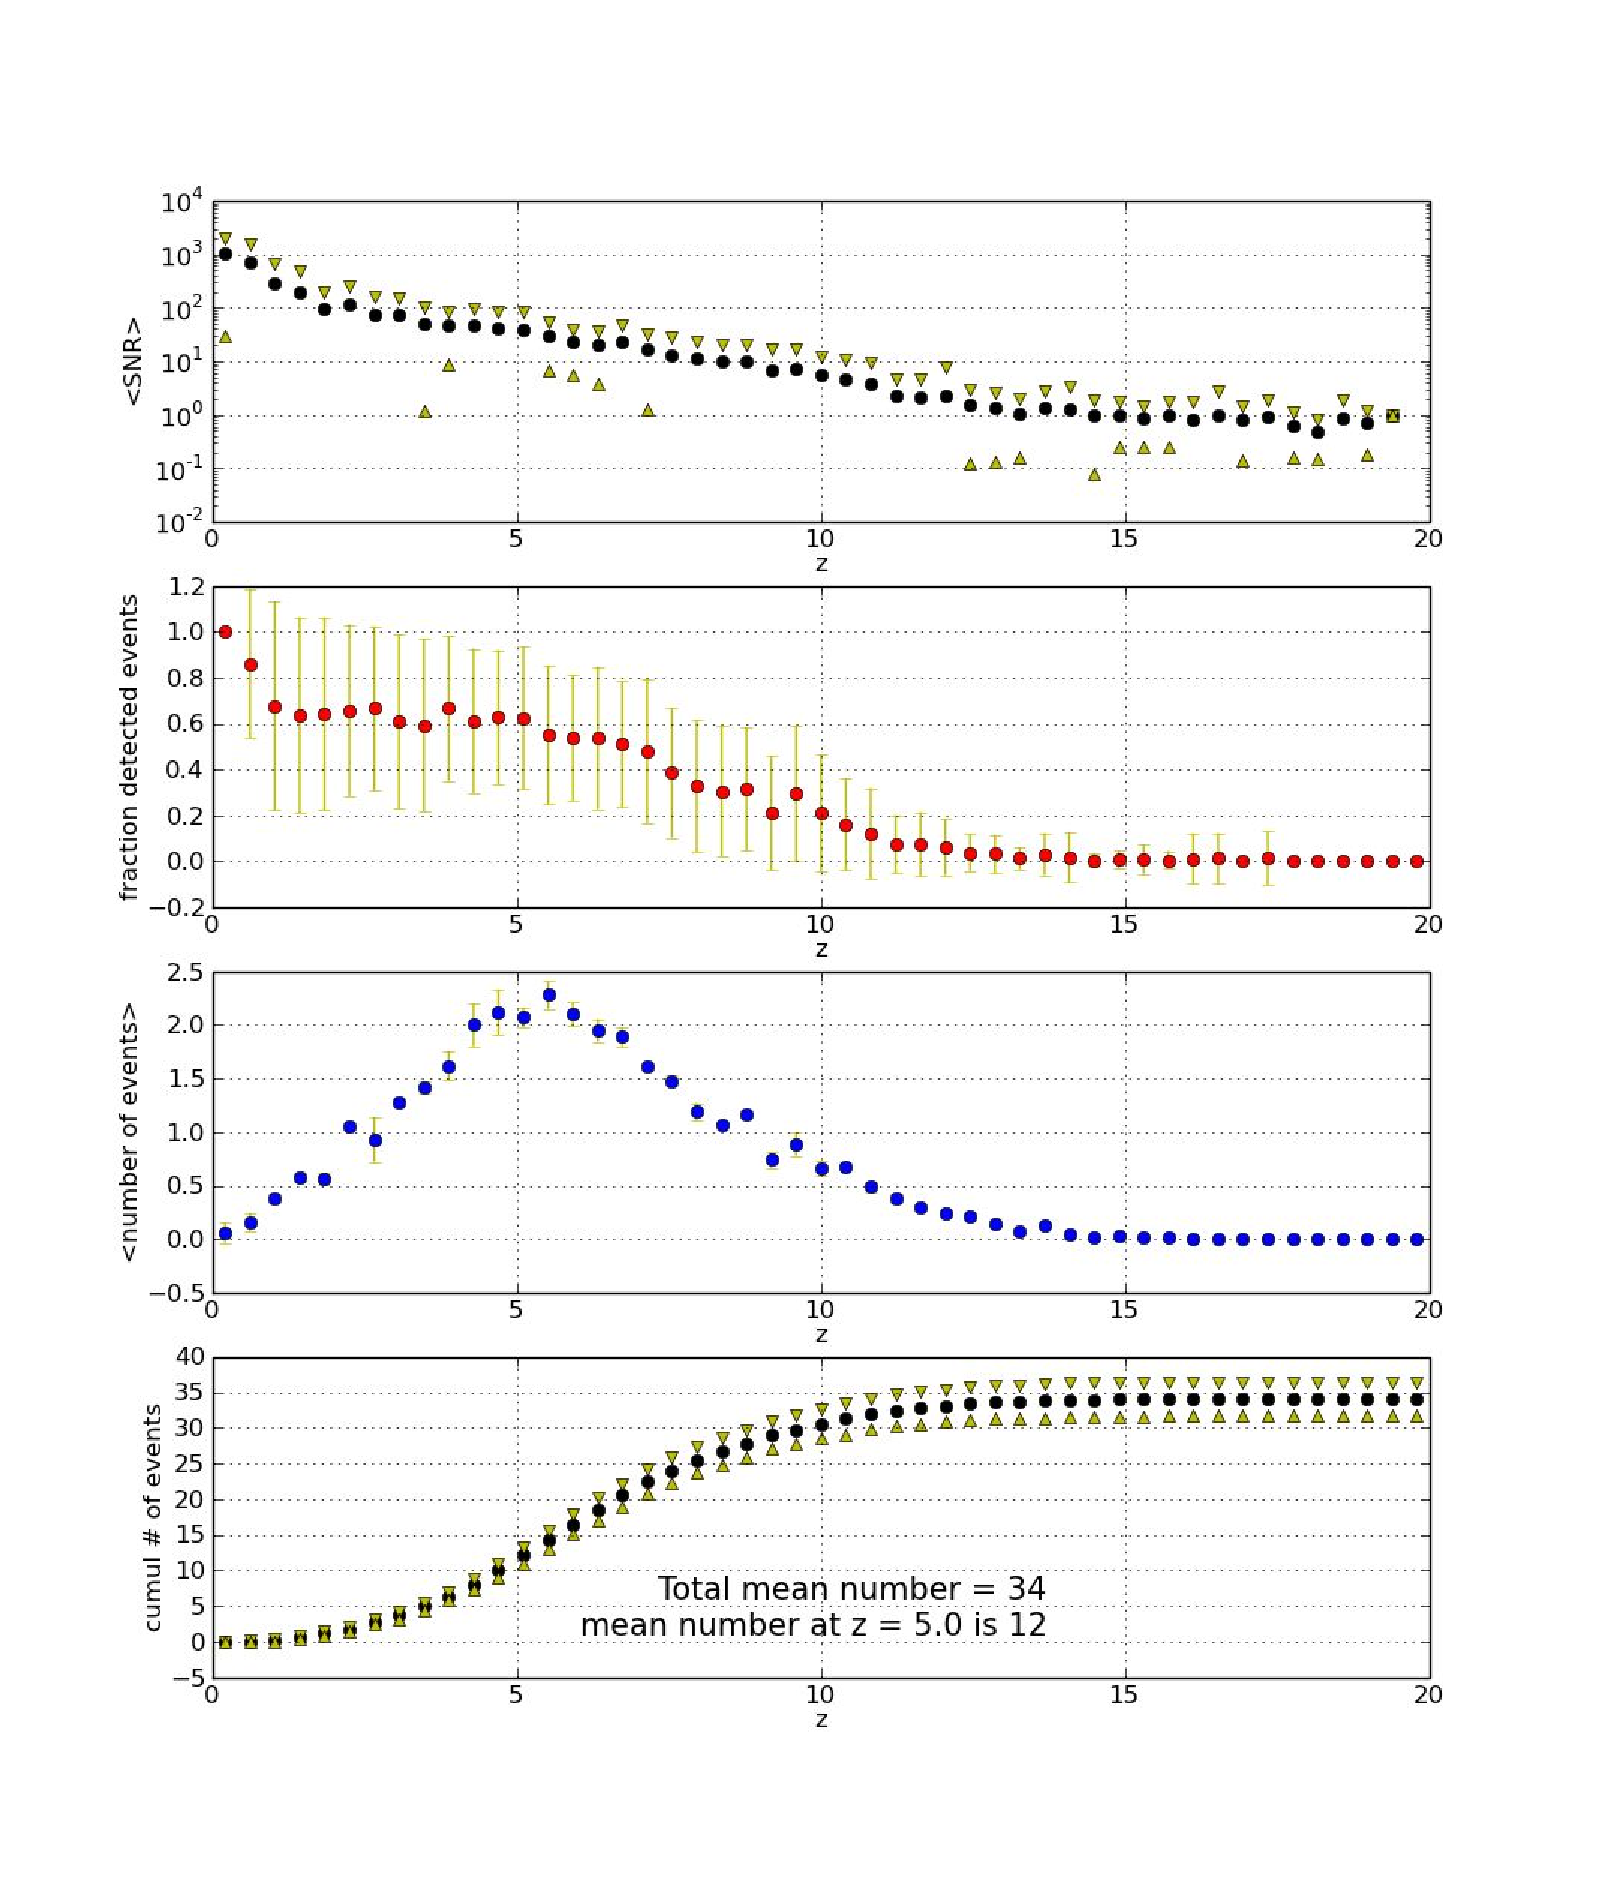
\includegraphics[scale=1,clip]{FigSMBHPhenomAEI/C2_mc_SNRs.eps}} 
\caption{Same as figure \ref{LISA_mc_SNR} but for C2.
\label{C2_mc_SNR} } 
\end{figure}


\begin{figure}
\resizebox{\hsize}{!}{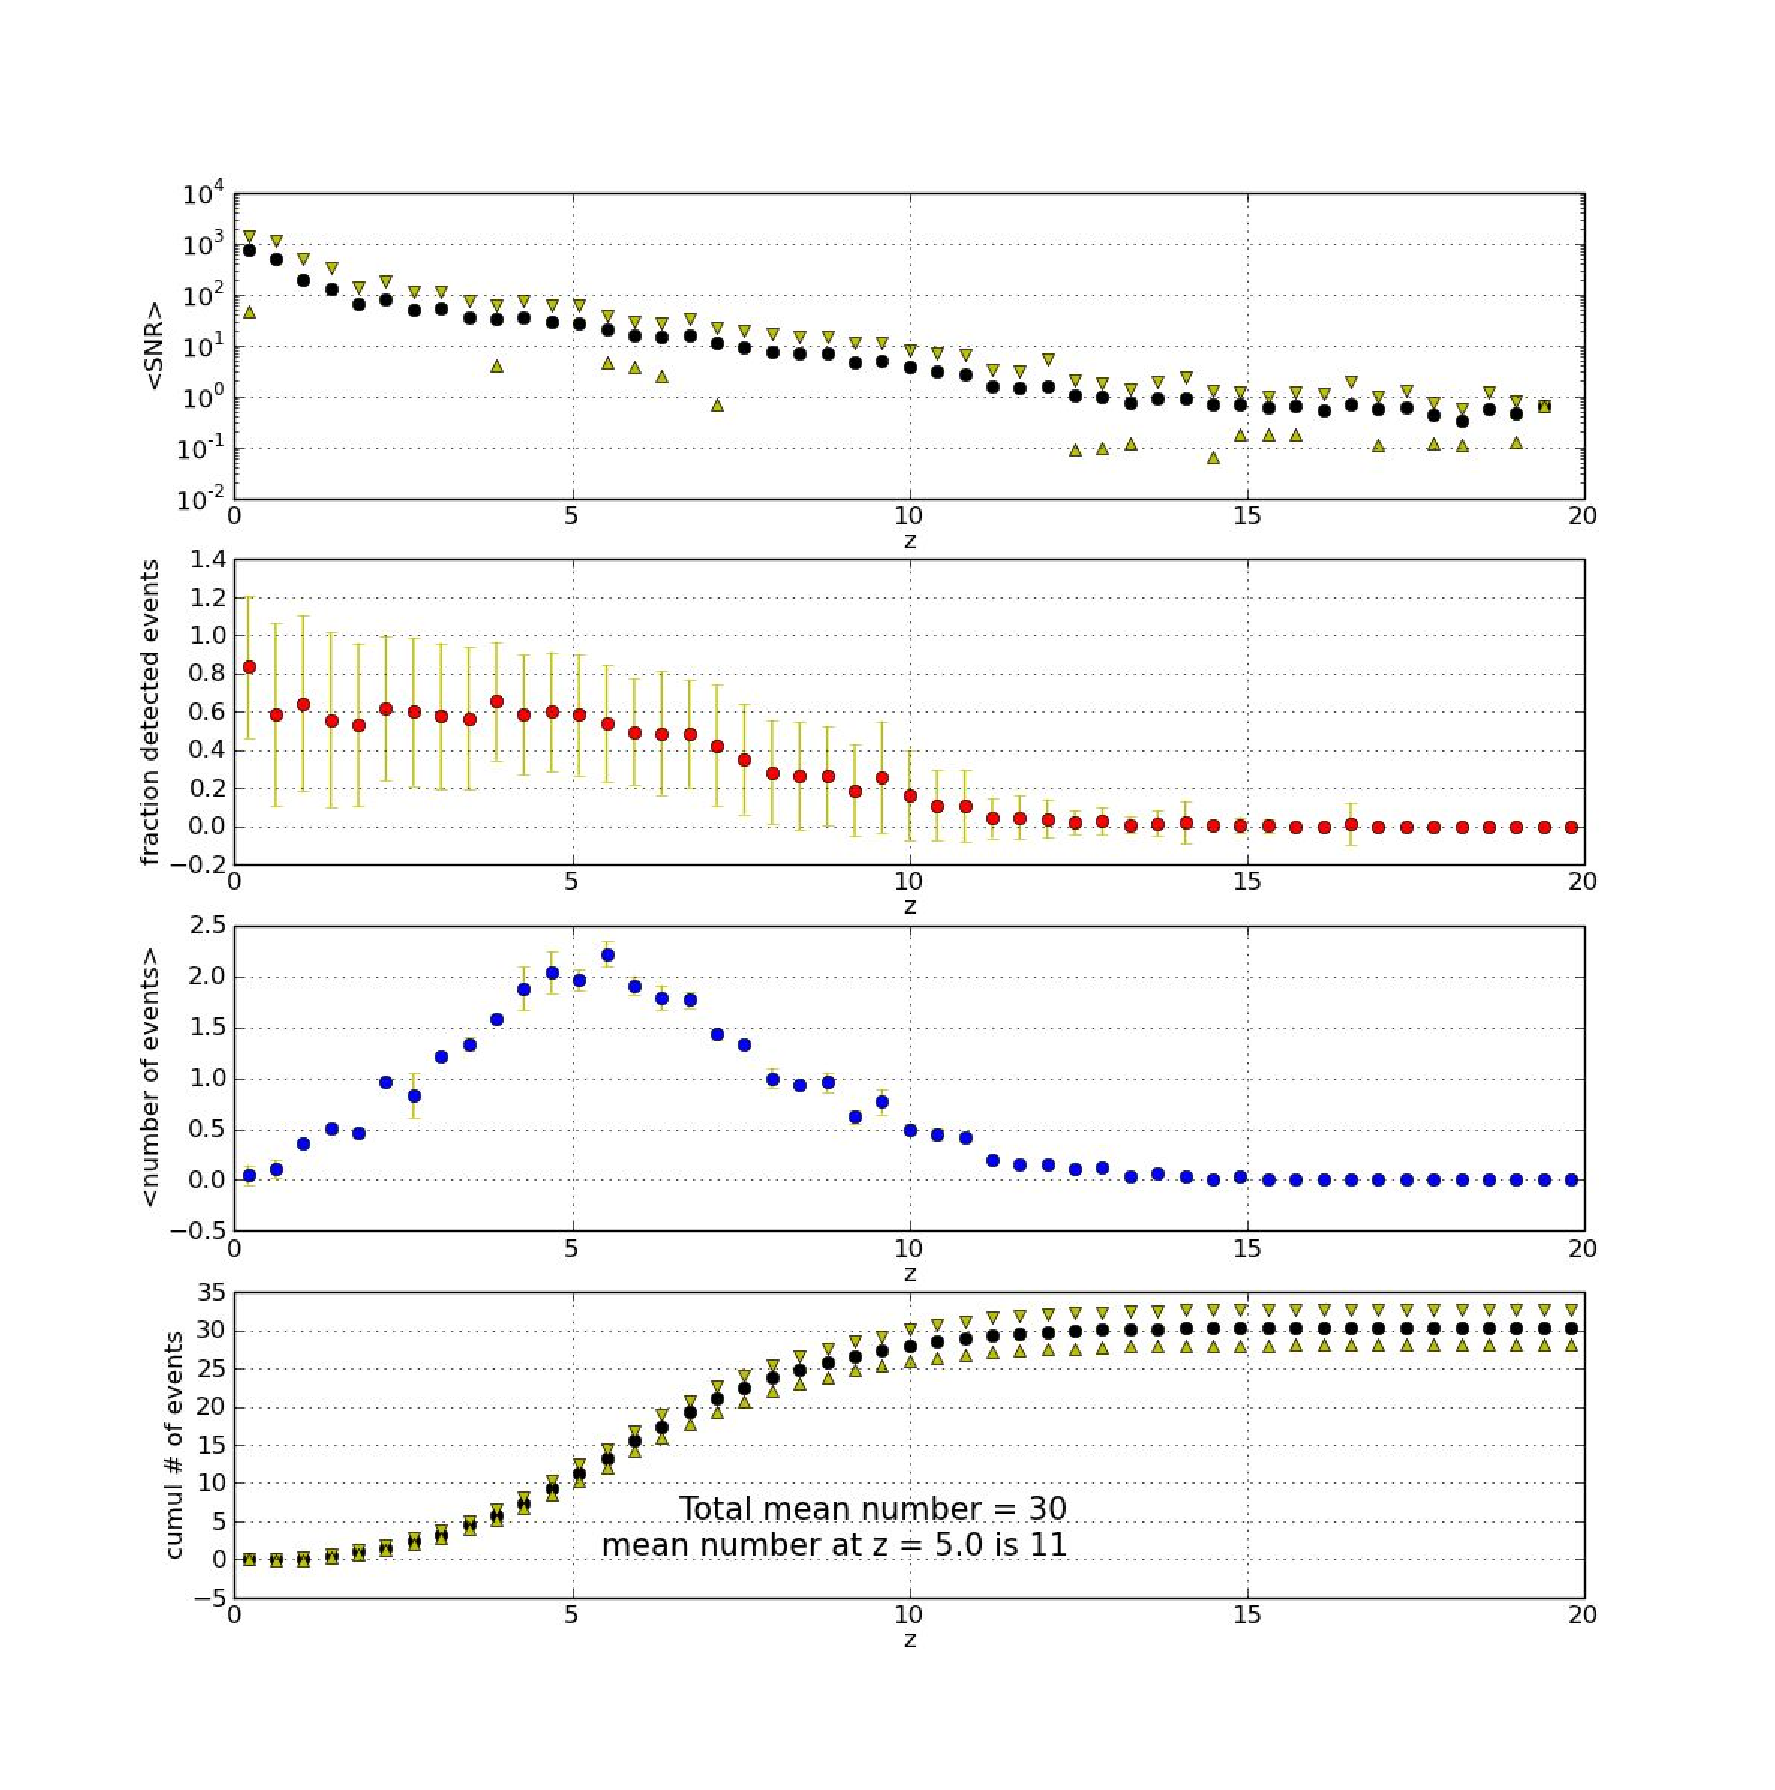
\includegraphics[scale=1,clip]{FigSMBHPhenomAEI/C1_mc_SNRs}} 
\caption{Same as figure \ref{LISA_mc_SNR} but for C1.
\label{C1_mc_SNR} } 
\end{figure}



%%%%%%%%%%%%%%%%  Histogram LISA, C1 and C3  %%%%%%%%%%%%%%%%


\begin{figure}
\resizebox{\hsize}{!}{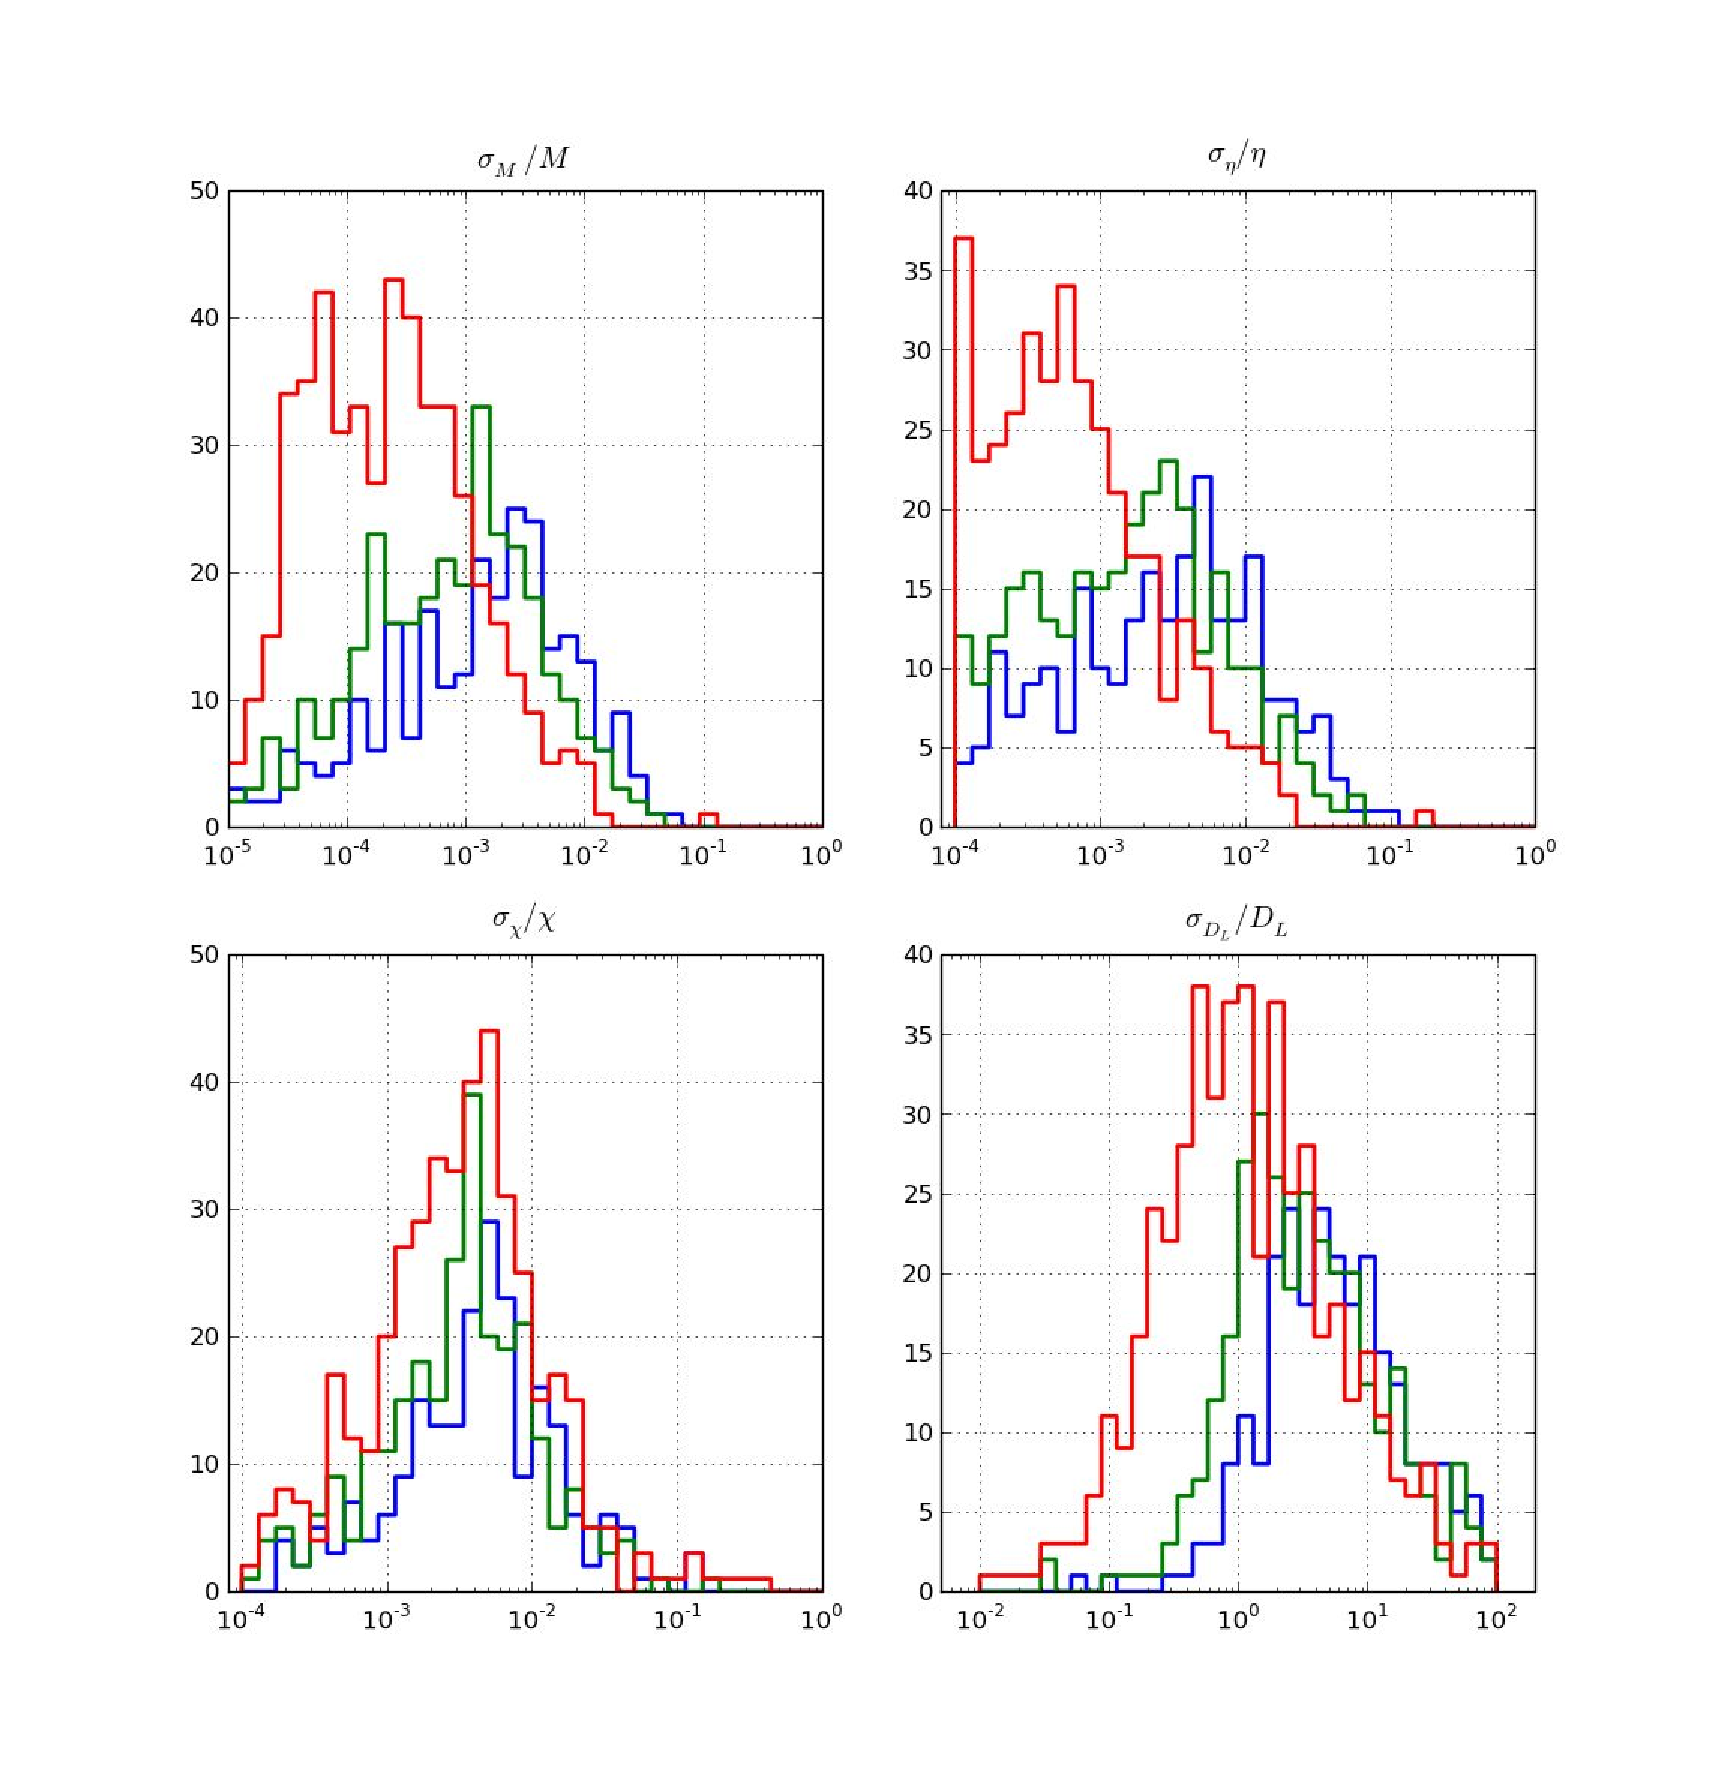
\includegraphics[scale=1,clip]{FigSMBHPhenomAEI/Hist_SE_LISAC1C2.eps}} 
\caption{1-$\sigma$ errors on source parameters: redshifted mass (upper left); symmetric mass ratio (upper right); spin parameter (lower left); luminosity distance (lower right). Histograms collect all the events in the SE catalogue, with SNR$>10$. Red histograms are for LISA, green histograms are for C2 and blue histograms are for C1.
\label{Hist_SE_LISAC1C2} } 
\end{figure}



\begin{figure}
\resizebox{\hsize}{!}{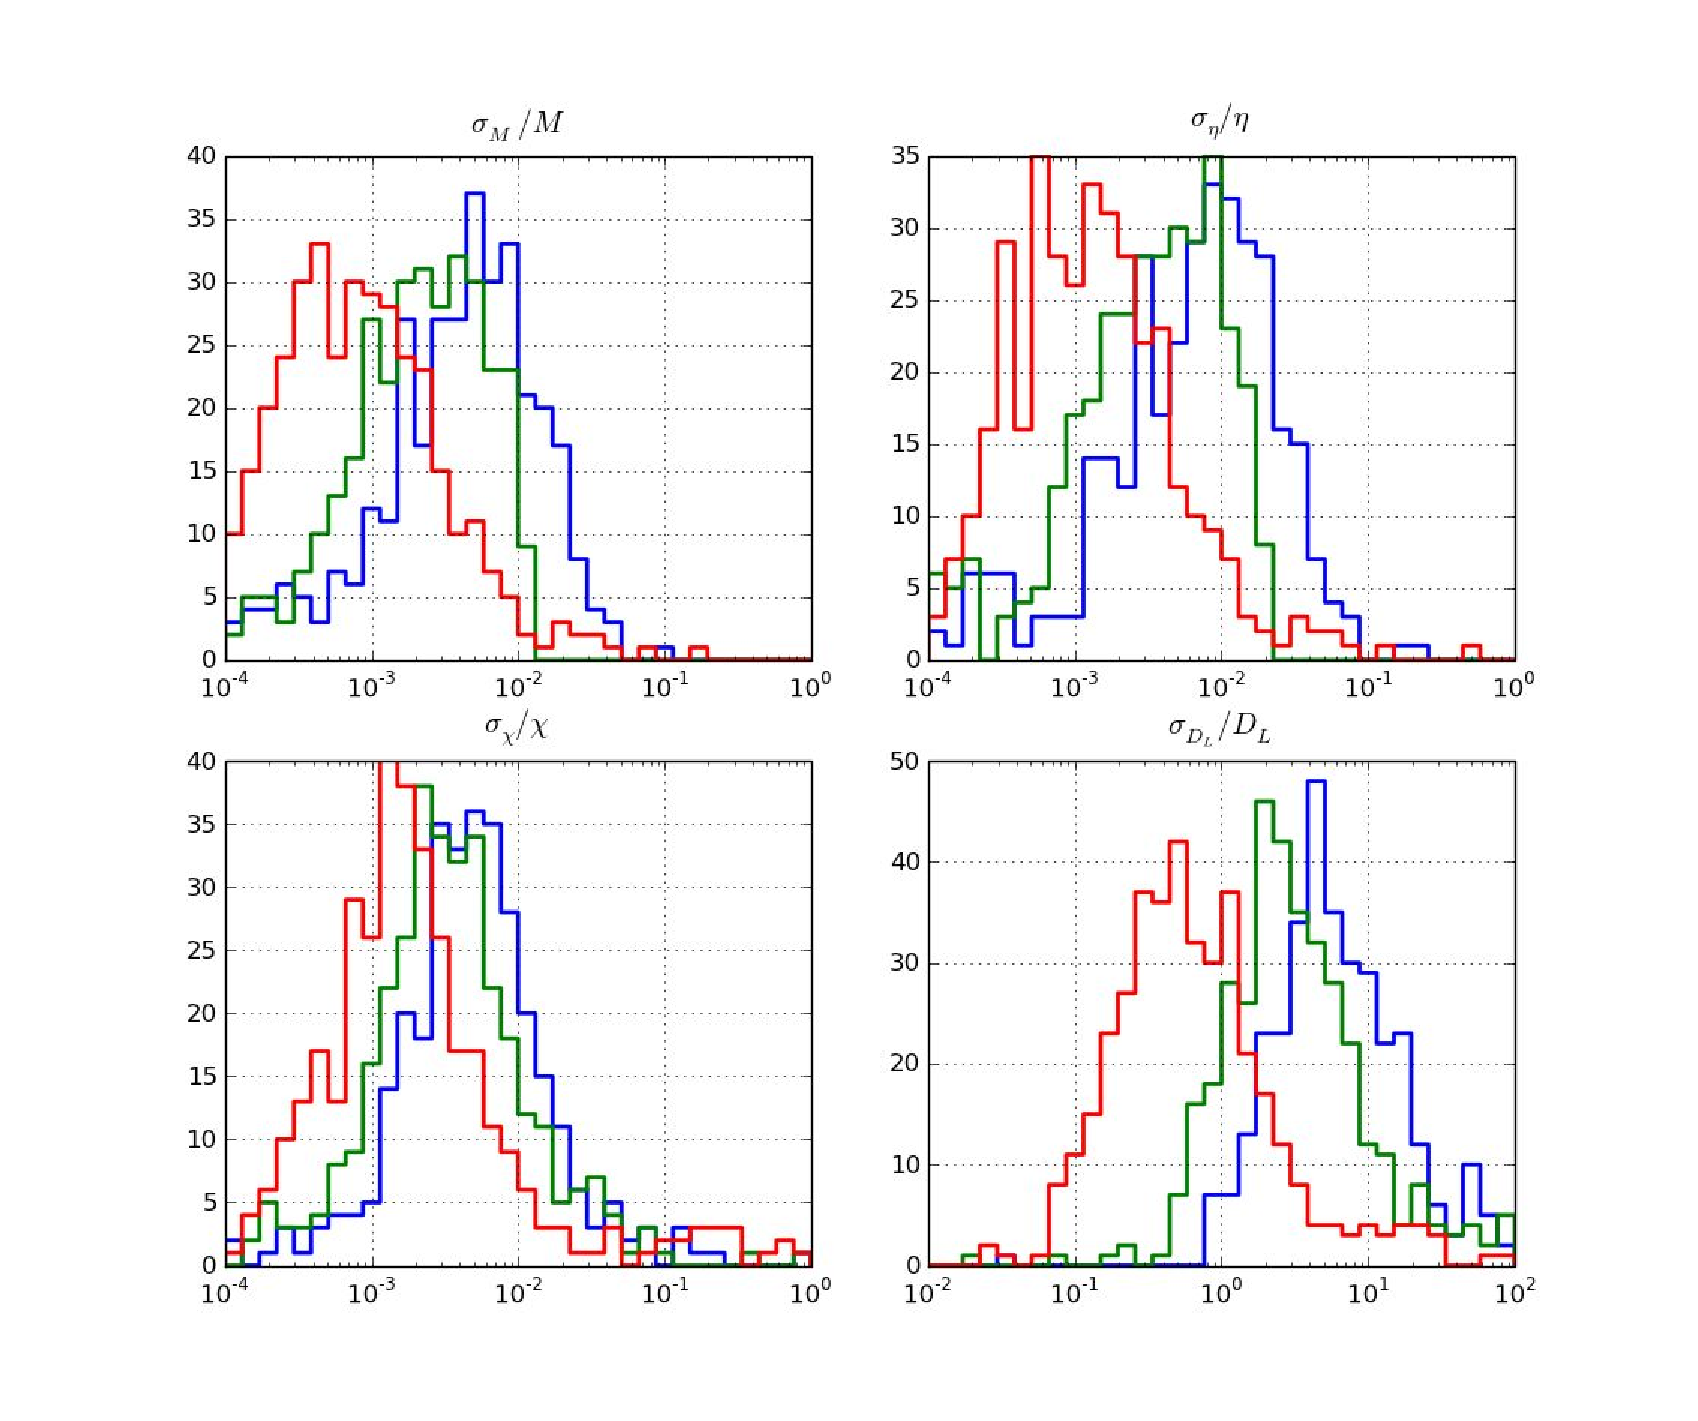
\includegraphics[scale=1,clip]{FigSMBHPhenomAEI/Hist_LE_LISAC1C2.eps}} 
\caption{Same as figure \ref{Hist_SE_LISAC1C2} but for the LE catalogue.
\label{Hist_LE_LISAC1C2} } 
\end{figure}


%%%%%%%%%%%%%%%%  Median erroe LISA, C1 and C3  %%%%%%%%%%%%%%%%


\begin{figure}
\resizebox{\hsize}{!}{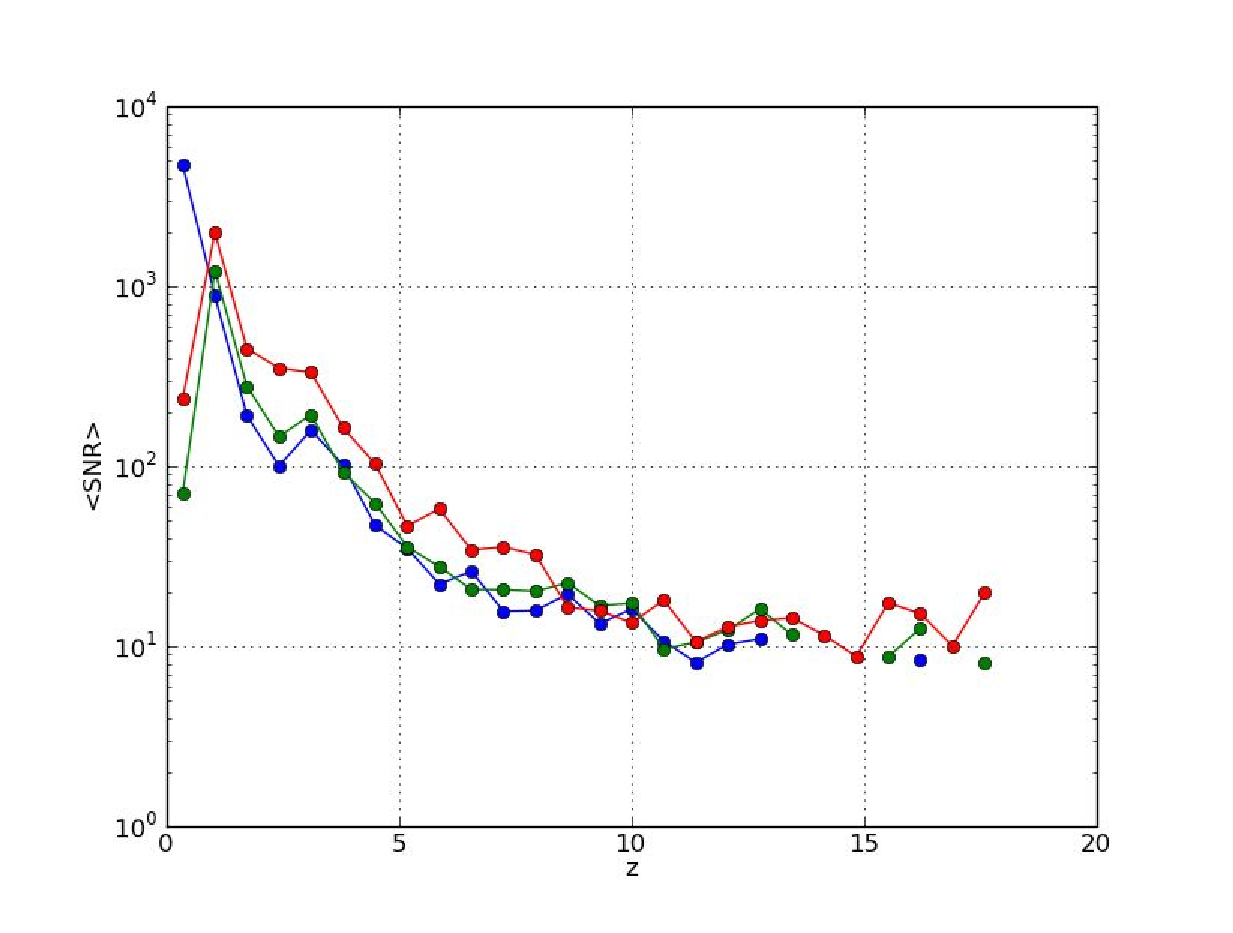
\includegraphics[scale=1,clip]{FigSMBHPhenomAEI/MedianSNR_SE_LISAC1C2.eps}} 
\caption{Median source SNR as a function of $z$. Colorstyle as in figure
\ref{Hist_SE_LISAC1C2}. Model SE is assumed.
\label{MedianSNR_SE_LISAC1C2} } 
\end{figure}



\begin{figure}
\resizebox{\hsize}{!}{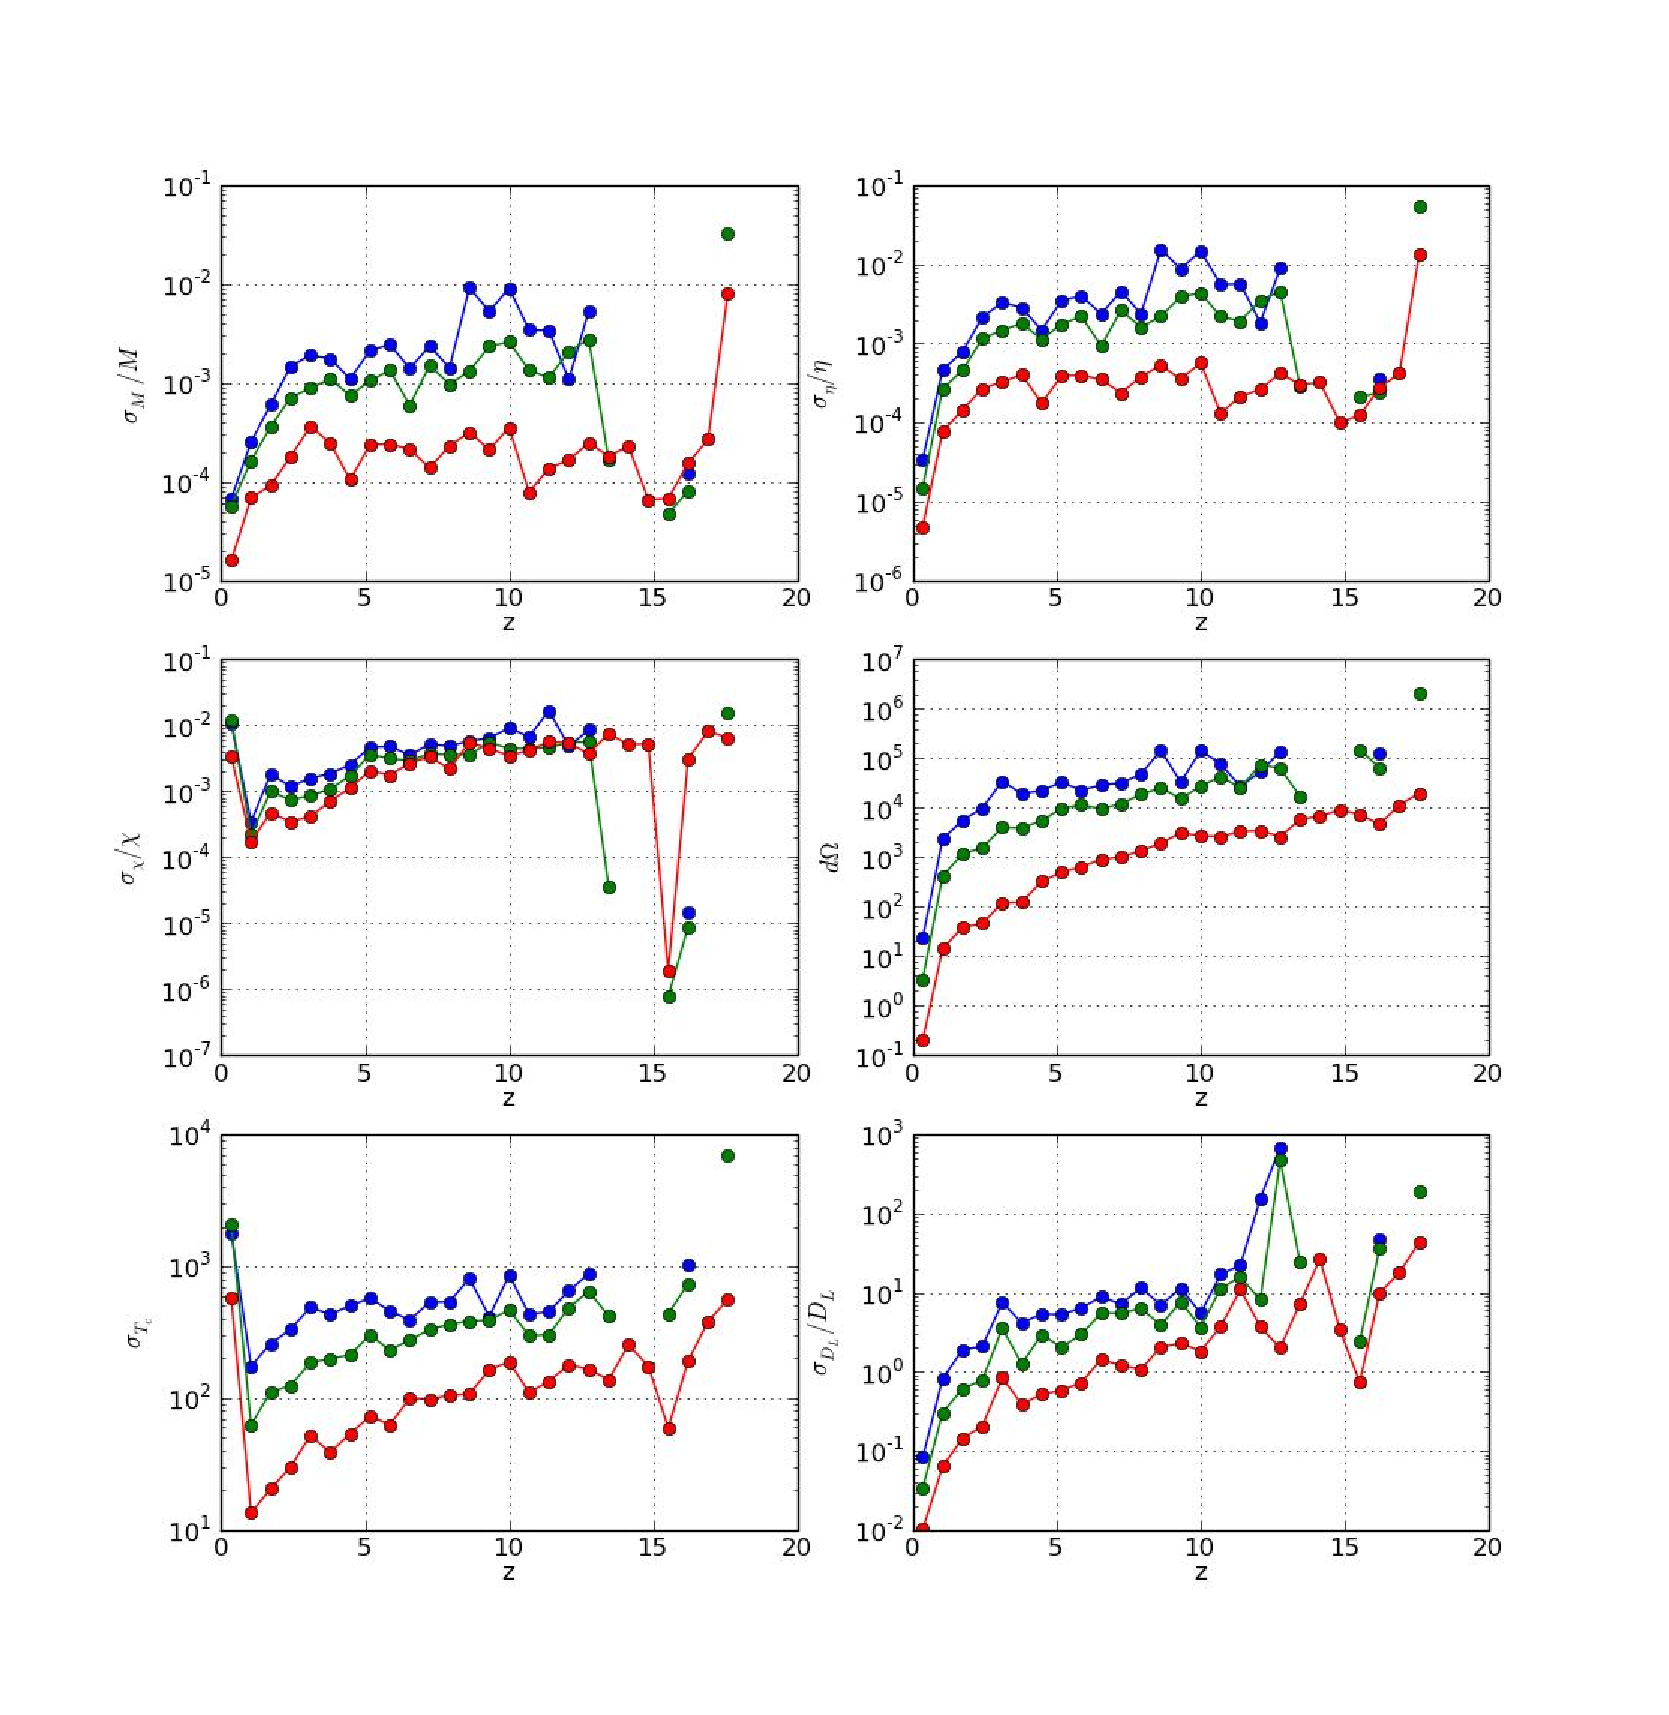
\includegraphics[scale=1,clip]{FigSMBHPhenomAEI/MedianErrs_SE_LISAC1C2.eps}} 
\caption{Median 1-$\sigma$ errors on the source parameters as a function of 
$z$: redshifted mass (upper left); symmetric mass ratio (upper right); spin parameter (middle left); sky location in deg$^2$ (middle right); coalescence time in seconds (lower left); luminosity distance (lower right). Colorstyle as in figure \ref{fig4}. Model SE is assumed.
\label{MedianErrs_SE_LISAC1C2} } 
\end{figure}



\begin{figure}
\resizebox{\hsize}{!}{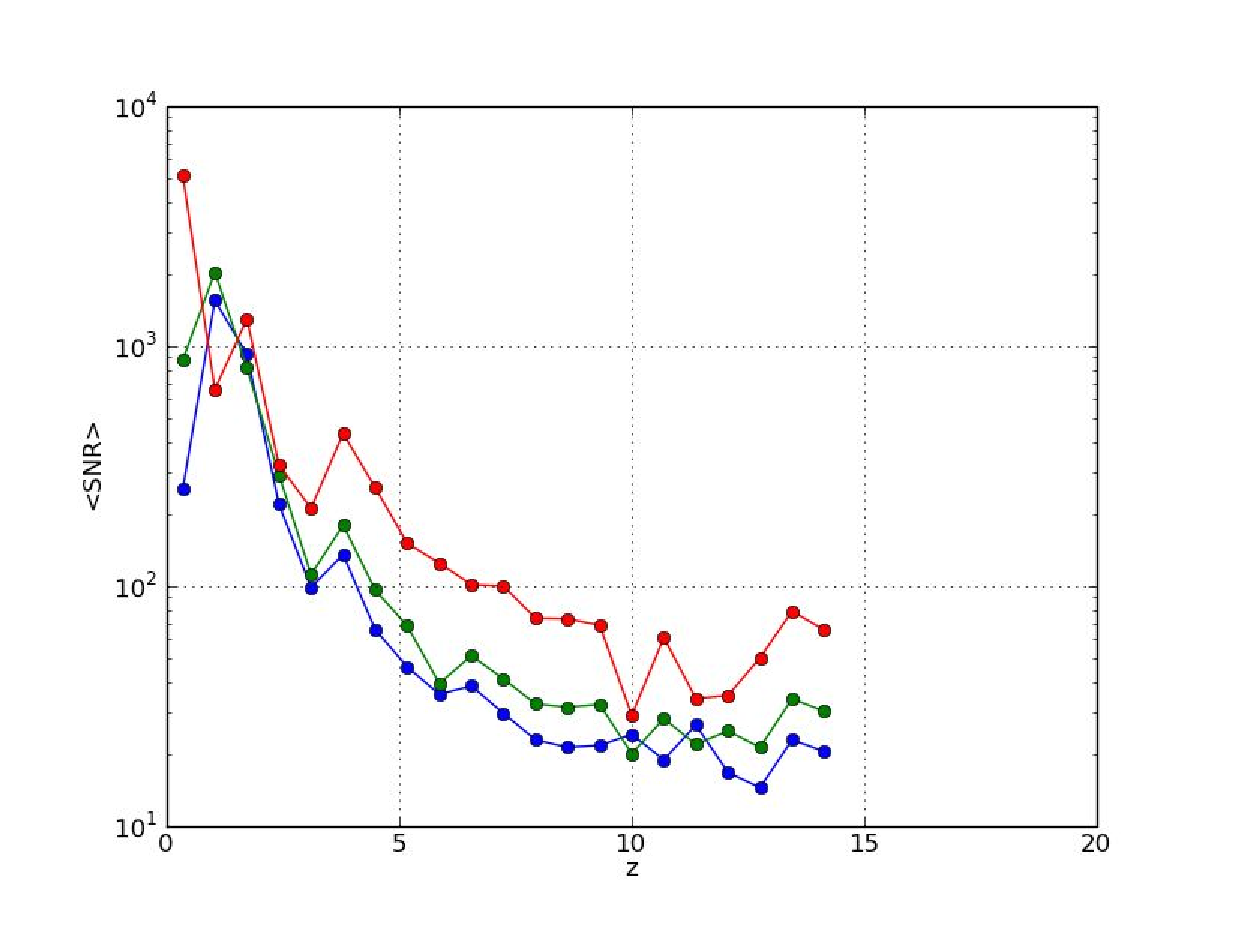
\includegraphics[scale=1,clip]{FigSMBHPhenomAEI/MedianSNR_LE_LISAC1C2}} 
\caption{Same as figure \ref{MedianErrs_SE_LISAC1C2} but for the LE catalogue.
\label{MedianSNR_LE_LISAC1C2} } 
\end{figure}



\begin{figure}
\resizebox{\hsize}{!}{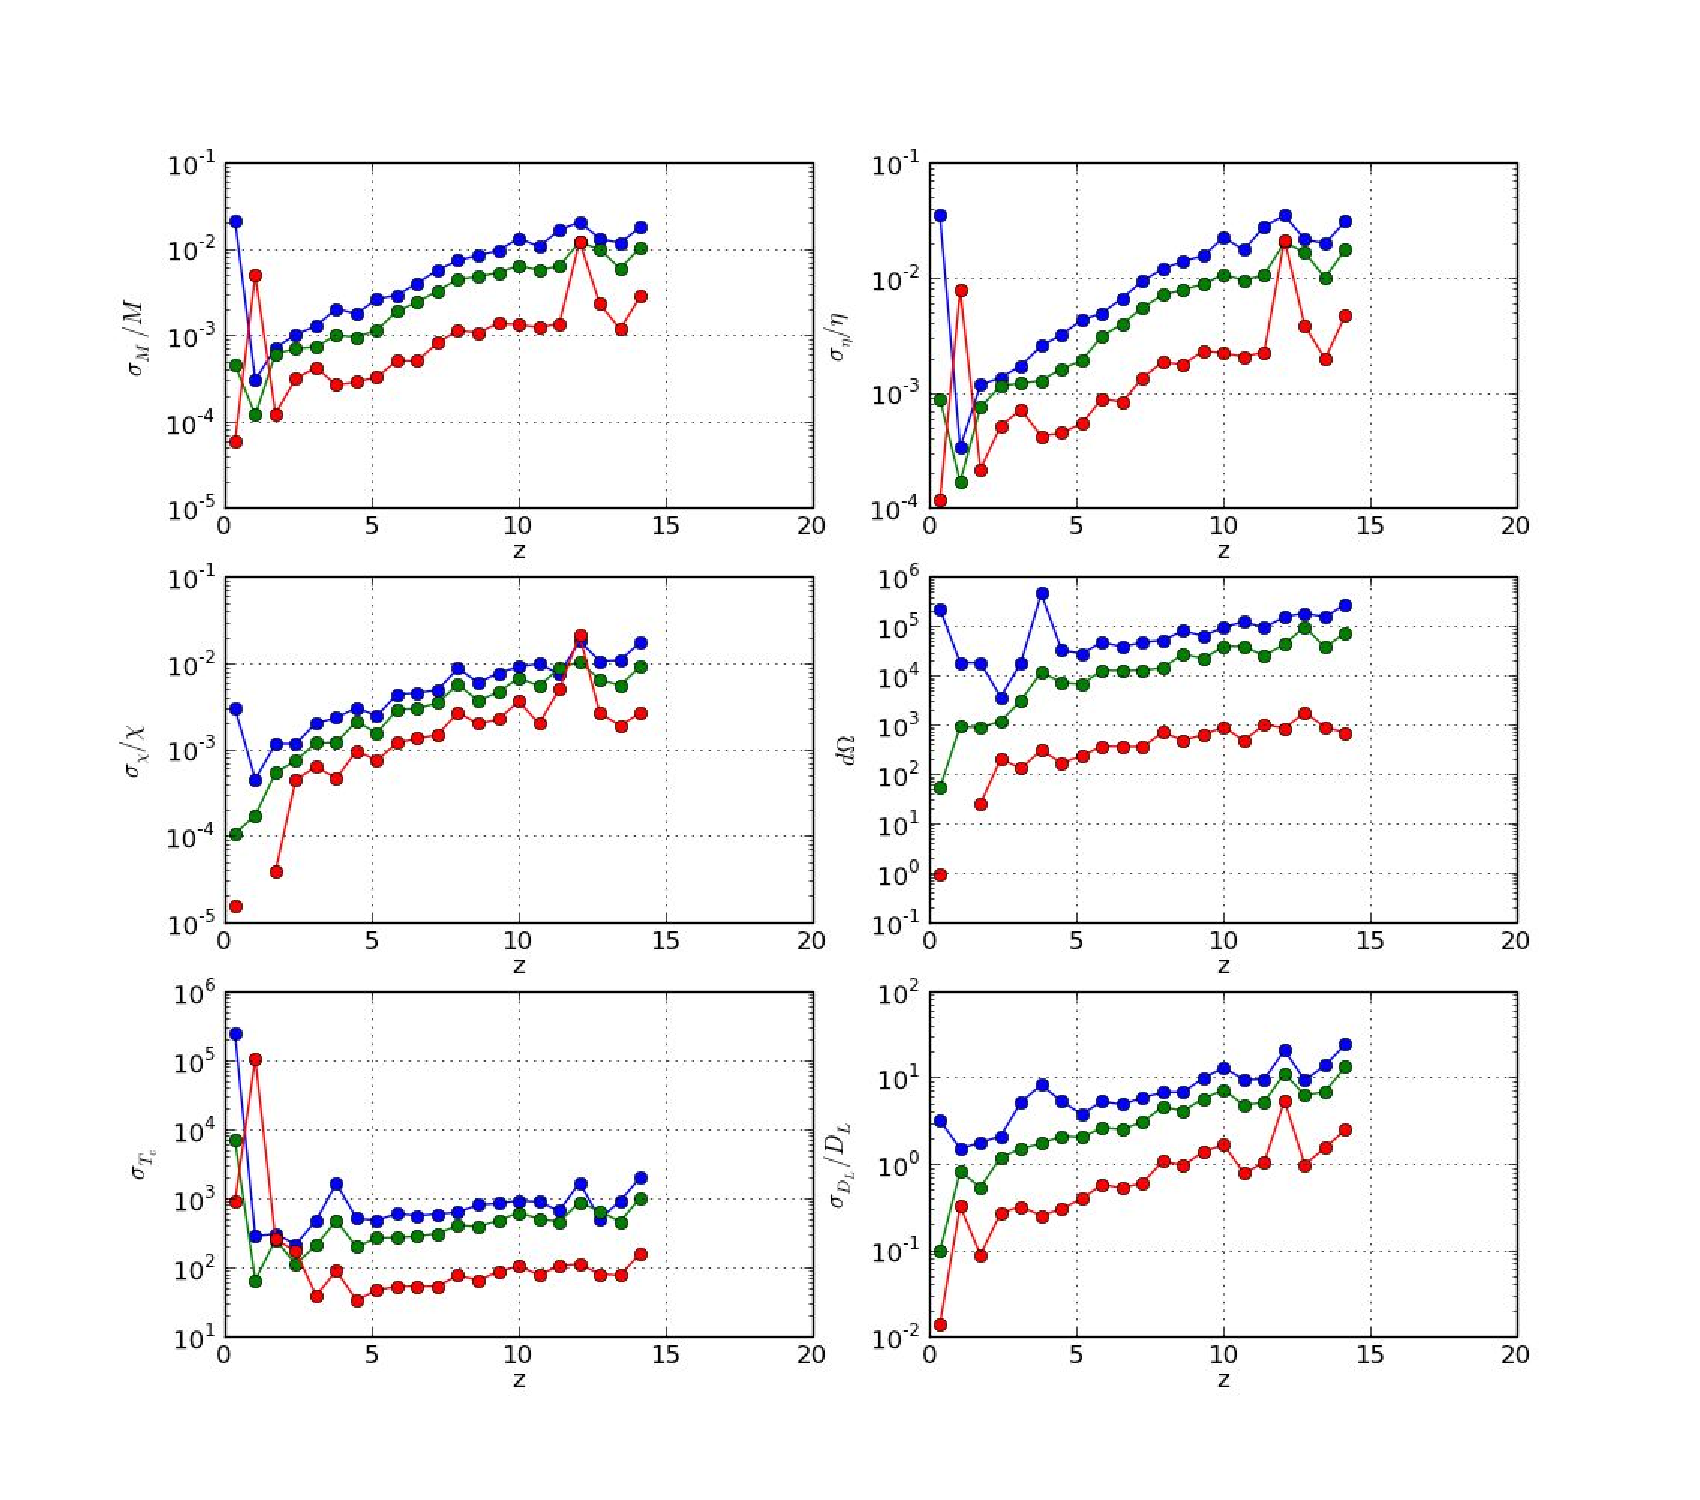
\includegraphics[scale=1,clip]{FigSMBHPhenomAEI/MedianErrs_LE_LISAC1C2}} 
\caption{Same as figure \ref{MedianErrs_SE_LISAC1C2} but for the LE catalogue.
\label{MedianErrs_LE_LISAC1C2} } 
\end{figure}















%%%%%%%%%%%%%%%    Model selection 
\subsection{Model selection}
\label{SS:MBHbModel}
{\it ('section captain' : Alberto Sesana) }
























%%%%%%%%%%%%%%%%%%%%%%%%%%%%%%%%%%%%%
%                                                            EMRIs                                                        %
%%%%%%%%%%%%%%%%%%%%%%%%%%%%%%%%%%%%%

\section{EMRIs}
{\it ('section captains' : Jon Gair \& Ed Porter) }

























\begin{thebibliography}{}

\bibitem{sm10}
L. Santamaria, F. Ohme, P. Ajith, B. Bruegmann, N. Dorband, M. Hannam, S. Husa, P. Moesta, D. Pollney, C. Reisswig, E. L. Robinson, J. Seiler and B. Krishnan,  Phys.\ Rev.\  D {\bf 82}, 064016 (2010)

\bibitem{dhu05}
{Dhurandhar}, S.~V. and {Nayak}, K.~R. and {Koshti}, S. and {Vinet}, J.-Y. Classical and Quantum Gravity {\bf 22}, 481-487 (2005)

\end{thebibliography}{}






\end{document}



